\documentclass{article}
\usepackage{graphicx}
\usepackage{wrapfig}
\usepackage{subcaption}
\usepackage[margin=1in]{geometry}
\usepackage{amsmath} % or simply amstext
\usepackage{amssymb}
\usepackage{siunitx}
\usepackage{booktabs}
\usepackage[export]{adjustbox}
\usepackage{cleveref}
\usepackage{booktabs}
\usepackage{gensymb}
\usepackage{float}
\usepackage[x11names,table]{xcolor}
\usepackage{setspace}
\usepackage[font=small]{caption}
\setstretch{1.5} % line spacing
\captionsetup[table]{font={stretch=1,small}} % line spacing in tables
\captionsetup[figure]{font={stretch=1,small}} % line spacing in figures
\usepackage{url}
% For timeline
\newcommand{\foo}{\color{LightSteelBlue3}\makebox[0pt]{\textbullet}\hskip-0.5pt\vrule width 1pt\hspace{\labelsep}}
\DeclareCaptionFont{blue}{\color{LightSteelBlue3}}
\usepackage{array,booktabs}

\title{PhD Research Proposal: Molecular Level Design of Nanoporous Lyotropic Liquid
Crystal Membranes for Aqueous Separations \\ \vspace{0.5cm}
\large Advisors: Michael Shirts and Richard Noble}

%MRS: overall, really nice start.  You can cut back a little on the detail and emphasize a bit more ``This is what the data means and what the consequnces are.  Need to flesh out objective 3 a more (and objective 4 a bit more). 
\author{Benjamin J. Coscia} 

\begin{document}

  \graphicspath{{./figures/}}

  \maketitle
  \thispagestyle{empty}
  \clearpage
  \setcounter{page}{1} % don't count title page as a page 

  \section{State of the Art}\label{section:state-of-the-art}

  \subsection*{Commercial Membranes for Small Molecule Separations}
  
  % perhaps a word or two about micro and ultra filtration  
  
  % re-word. This paragraph is verbatim from structure paper
  More highly selective nanoporous membranes would be useful for 
  performing complex aqueous separations with seawater and various
  types of wastewater.

  %MRS: probably can do a little less introduction of the overall membrane needs, as we want to make sure 
  %MRS: the focus is on the research (thesis, you can include everything).  Can probably hold off that until you get the rest done, then trim as needed for space.
  %
  %MRS: remember the purpose of the introduction to any document is to lay out the rules of engagement; you want 
  %MRS: to raise the questions that the rest of the document will answer.
  % 
  %MRS: try to make sure the application motivation and the research described match up when possible.
  %MRS: if particular applications wouldn't be directly enabled by the research, at least draw to the connection
  %MRS: i.e. talk about the general tools of computation to understand nanostructured membranes, even if the current
  %MRS: membranes under development aren't suitable for the particular separations described.
  \begin{itemize}
    \item For example, sodium chloride and boron in seawater 
    \cite{fritzmann_state---art_2007} and organic micropollutants found in
    municipal and industrial wastewaters \cite{schwarzenbach_challenge_2006}
    represent just a few of the diverse contaminants of water sources. 
    \item By efficiently separating contaminants from feed solutions with
    highly selective membranes, it is possible to reduce the number of 
    required membrane passes and post-treatment steps needed for a given 
    filtration process \cite{werber_materials_2016}, thus lowering cost
    and energy requirements. 
    \item Additionally, one can extract valuable resources from the 
    feed streams. For example, flowback water produced during hydraulic
    fracturing of shale formations contains dissolved species such as acetate
    whose extraction has economic value \cite{dischinger_application_2017}.
  \end{itemize}

  Reverse osmosis (RO) and nanofiltration (NF) are two prevailing membrane
  filtration processes that can be used to separate solutes on the order of
  1 nm in size and smaller, including ions.
  \begin{itemize}  
    \item Both apply hydraulic pressure to the feed solution in order to 
    overcome osmotic pressure and force water and unfiltered components 
    through the membrane.
    \item RO membranes are typically thin film composite with a porous mechanical 
    support layer and a thin but dense polymer matrix active layer where separations
    occur.\cite{jeong_interfacial_2007}
    \item RO separates solutes based on the solute's ability to dissolve into
    and diffuse through the tortuous pathways available in the membrane's dense 
    active layer.
    \item RO offers high selectivity at the cost of relatively high energy 
    requirements since one must apply hydraulic pressure of up to 100 bar in 
    order to achieve an economical flux~\cite{van_der_bruggen_review_2003}.  % get number
    \item In contrast to RO membranes, NF membranes have explicit pores on the
    order of 1 nm in size. 
    \item Typically, separations are achieved based on size exclusion and
    charge exclusion if the membrane's surface has a net charge.
    \item NF membranes require significantly less applied pressure in order
    to achieve solute flux comparable to RO.
    \item Unfortunately, conventional synthesis processes, such as 
    phase-inversion\cite{smolders_microstructures_1992} are stochastic in
    nature which yields pores that are polydisperse in size.\cite{werber_materials_2016} % name some synthesis processes
    \item Pore size polydispersity is detrimental to membrane selectivity
  \end{itemize}
  
  The downfall of RO and NF membranes can be summarized by the well-known
  permeability-selectivity tradeoff. Namely, it is difficult to increase the
  permeability of a desired molecular or atomic species, while maintaining
  the same retention of an undesired species.\cite{werber_materials_2016}  
  
  \subsection*{Nanostructured Membranes}
  
  Nanostructured membranes attempt to overcome the permeability-selectivity 
  tradeoff through intelligent design at the molecular level.
  \begin{itemize}
	\item Graphene sheets, carbon nanotubes (CNTs) and zeolites are three
	highly studied nanostructured technologies.
  \end{itemize}
  
  Ultrathin-film graphene and graphene oxide membranes are a very active
  area of research because they offer potential for extremely high 
  permeability membranes.
  \begin{itemize}
    \item An ideal graphene membrane is a 2D material consisting of a
    single layer of graphene.\cite{humplik_nanostructured_2011}
    \item Synthesis of a single layer of graphene at a large scale without
    introducing defects is a challenge that has not yet been overcome.
    \item Multilayered graphene membranes are a potentially easier and
    more scalable technology which has garnered increasing interest in
    recent years.\cite{cohen-tanugi_multilayer_2016,wei_multilayred_2018}
  \end{itemize}
  
  Carbon nanotubes (CNTs) have shown promise as aqueous separations membranes due
  to unprecedentedly fast water transport.\cite{humplik_nanostructured_2011,hummer_water_2001} 
  \begin{itemize}
    \item Practically, dispersing CNTs into a polymer matrix is extremely difficult
    because they tend to agglomerate due to Van der Waals forces.
    \item Functionalization of the CNT walls has been heavily investigated 
    as a way to overcome this issue. 
    \item Alignment of the CNTs into an array feasible as a nanoporous
    membrane presents a further challenge to CNT membranes.\cite{sahoo_polymer_2010}
  \end{itemize}
   
  Zeolite-coated ceramic membranes offer the potential for permeabilities
  comparable to ultrafiltration with selectivities as good as NF and RO. 
  \begin{itemize}
    \item Zeolites have highly uniform nm-sized crystalline structures with
    cage-like cavities that allow movement and trapping of small solutes. 
    \item The crystalline frameworks are typically formed by networks of silicon
    and aluminum each attached to 4 oxygen atoms in a tetrahedral arrangement. 
    \item One can replace the silicon and aluminum atoms via ion exchange 
    in order to control the size of the cavities and hence its molecular-seiving properties.
    \item A number of studies have tested the permeability and sodium salt
    rejection of various zeolite membranes, however none have fully
    overcome the permeability-selectivity tradeoff.
    \item Most are prone to defects in the crystalline structure.\cite{pendergast_review_2011}
  \end{itemize}

  \subsection*{Lyotropic Liquid Crystal Membranes}
  
  Preliminary evidence has shown that cross-linked lyotropic liquid crystal
  (LLC) membranes can be produced at moderate scale and may be capable of 
  performing highly selective separations. 
  \begin{itemize}  
    \item LLCs are amphiphilic molecules that have the ability to self-assemble
    into porous nanostructures\cite{smith_ordered_1997} that
    can be cross-linked to create mechanically strong membrane films with 
    periodic uniform-sized pores on the order of 1 nm in diameter \cite{zhou_supported_2005}. 
    \item Since LLC polymer membranes lack an appreciable pore size distribution,
    they inherently exhibit high selectivity due to their strict molecular weight
    cut-off (MWCO)~\cite{zhou_supported_2005}. 
    \item Additionally, LLC monomers can be salts, and therefore lead to Donnan
    exclusion of ions in solution.\cite{donnan_theory_1995}
%    The membrane gains a net surface charge when counterions from
%  the head groups that line the pore walls escape into the feed solution in an
%  effort to balance the gradients of concentration and electric potential
%  \cite{donnan_theory_1995}.
  \end{itemize}

  The feasibility of nanostructured LLC polymer membranes for selective separations
  has been demonstrated using LLC monomers that form the type 1 bicontinuous cubic
  (Q\textsubscript{I})\cite{hatakeyama_water_2011,hatakeyama_nanoporous_2010,carter_glycerol-based_2012}
  and the inverted hexagonal (H\textsubscript{II}) \cite{zhou_supported_2005}
  phases. 
  \begin{itemize}
    \item When separating organic solutes from NaCl, Q\textsubscript{I}-phase
    membrane filtration experiments have shown selectivity 2--3 times higher than
    commercial RO and 6--12 times higher than commercial NF membranes.\cite{dischinger_application_2017}
    \item When separating a series of various sized dyes, the 
    H\textsubscript{II}-phase membrane showed complete rejection of dyes bigger
    than 1.2 nm in size \cite{zhou_supported_2005}.
  \end{itemize}

  Q\textsubscript{I}-phase membranes consist of a tortuous network of three
  dimensionally interconnected pores that prevent optimal through-plane
  transport. 
  \begin{itemize}
    \item In contrast, the densely packed, non-tortuous and uniform sized
    pores of H\textsubscript{II}-phase membranes represent the ideal geometry
    for achieving high solute flux\cite{matyka_tortuosity-porosity_2008}.  
    \item However, the hexagonally packed LC domains of the H\textsubscript{II}-phase
    generally form mutually unaligned domains, which hurts membrane permeability. 
    \item This domain scale misalignment had inhibited further development of 
    this technology, and research efforts were focused on the Q\textsubscript{I}
    phase, whose geometry does not require alignment~\cite{zhou_new_2007}.
  \end{itemize}

%  The H\textsubscript{II}-phase pore geometry (Figure~\ref{fig:assembly}) has a
%  high theoretical capacity for transport than the Q\textsubscript{I} phase.
%  \begin{itemize}
%	  \item The H\textsubscript{II} phase forms at room temperature in the 
%	  presence of ca.~10 wt\% water and consists of hexagonally packed, 
%	  hydrophilic pore columns\cite{smith_ordered_1997}. 
%%	  \item The hexagonal, straight-pore geometry provides a dense array
%%	  of hydrophilic channels and short pathways for solutes to travel.
%	  % BJC: should rethink the following since we think that thermotropic doesn't exist
%	  \item In the absence of water, neat monomer will form the same hexagonal
%	  columnar structure which, in the literature, has been referred to as the
%	  Col\textsubscript{h} thermotropic phase\cite{feng_scalable_2014}.
%  \end{itemize}

  Recently, researchers have learned how to macroscopically align the
  hexagonal domains which has revived research into H\textsubscript{II}-phase LLC
  polymer membranes. 
  \begin{itemize}
    \item In 2014, Feng et al.~showed that one can align Col\textsubscript{h}
    domains, a temperature-dependent hexagonal phase created by neat LLC monomers,
    using a magnetic field with subsequent cross-linking to lock the structure 
    in place\cite{feng_scalable_2014}.
	\item In 2016, Feng et al.~showed that one could also obtain the same result
	by confining the neat monomer between PDMS or glass substrates since hexagonal
	mesophases preferentially anchor perpendicular to both surfaces\cite{feng_thin_2016}.
  \end{itemize}
  
  Unfortunately, reproducing the work of Feng et al. with the hydrated 
  H\textsubscript{II} phase has been an experimental challenge. Therefore, the
  primary focus of experimental research efforts has been with the Q\textsubscript{I} phase.

  \section{Project Objectives}\label{section:objectives}  
  
  Our current understanding of the molecular details of LLC membranes'
  nanostructure is not sufficient to be able to precisely design them for
  specific separations. 
  \begin{itemize} 
%    \item Over the past 20 years, H\textsubscript{II}-phase LLC polymer 
%    membrane studies have been limited primarily to the Na-GA3C11 monomer
%    with some characterization done after minor structural modifications.\cite{zhou_supported_2005,resel_structural_2000}
    \item Dischinger et al.~attempted to use an empirical model
    that correlates the physiochemical properties of the counterion used in
    a Q\textsubscript{I}-phase LLC membrane to solute rejection.\cite{dischinger_effect_2017}
    \item Although their model showed some qualitative agreement with experiment, the
    quality of fit of their model was limited due to complex solute-membrane
    interactions that could not easily be modeled. 
  \end{itemize}

  A molecular-level understanding of structure and transport in LLC polymer 
  membranes, enabled by molecular dynamics (MD) simulations, can provide 
  guidelines to reduce the large chemical space available to design
  monomers for creation of separation-specific membranes. 
  \begin{itemize}
    \item Using a sufficiently accurate molecular model, we can directly 
    observe transport of solutes within LLC membrane nanopores and infer
    mechanisms. 
    \item Based on this information 
%MRS: maybe ``will have a much greater capability''.  'can' is strong. 
we can intelligently design new membranes
    by screening new liquid crystal monomer designs.
    \item Our most promising designs can be tested experimentally.
%MRS: above: more likely, the principles learned can be implemented experimentally - that's much easier than full design.
  \end{itemize}
  
  \noindent There are four primary objectives of this PhD research.
  \begin{enumerate}
  
    \item Develop techniques to build and understand the nanoscopic structure
    of LLC membranes.

    %MRS: probably should talk about this 1) with proper tense (some of these things have been done) and 2) talk about what YOU are doing, not we. I helped design the research, but you carried essentially all of it out! If phrased in future tense, committee will be confused, thinking those are things still to be done.  

    Useful molecular-level modeling should incorporate a detailed picture 
    of the nanoscopic pore structure, which is crucial to understanding
    the role of monomer structure in solute transport and membrane design.
    We will generate simulated X-ray diffraction (XRD) patterns from MD trajectories
    and compare them to an experimental 2D wide angle X-ray scattering (WAXS)
    spectrum of a Col\textsubscript{h} phase membrane. We will assess the extent
    to which we can apply our understanding to the H\textsubscript{II} phase,
    as well as systems built with alternate monomers.
    
    \item Determine dominant solute-membrane interactions that give rise to
    transport mechanisms.
    
    We will observe transport of a relatively large set of small polar solutes
    placed within the H\textsubscript{II} membrane nanopores. We will observe
    the time series of each solute's position as well as directly measure the
    physical interactions, such as hydrogen bonding and ion coordination, 
    between solutes and LLC monomers.
    
    \item Create a stochastic model which can project long timescale 
    transport behavior.
    
    We will combine our general knowledge of the solute transport mechanisms
    with simulation data in order to inform a stochastic model. This model
    should closely reproduce the time series that we observe in our simulations.
    Due to the low computational cost of a stochastic model relative to 
    MD simulations, we will be able to project long timescale transport behavior
    and make well-converged predictions of macroscopic transport properties.
           
    \item Adapt the same analysis to the Q\textsubscript{I} phase.
    
    Over the course of this project, experimental research surrounding
    LLC membranes has shifted nearly all focus towards the Q\textsubscript{I}
    phase due to its more facile synthesis.	Although most of our work has 
    been applied to the H\textsubscript{II} phase, we expect that much of 
    the same analyses can be applied to the Q\textsubscript{I} phase. The 
    biggest challenge will be adapting our techniques to its more complex
    geometry.
    
%    \item Enable easy continuation of our work with a dedicated and 
%    well-documented python package.
%    
%	Although molecular simulations have become popular
%	for studying systems at the atomic level, LLCs used in this context
%	have not been heavily investigated. Consequently, much of the 
%	analysis developed for this project is not widely applied. Therefore, 
%	it is important for us to make available the scripts that reproduce
%	the exact results presented in our published papers along with detailed
%	documentation of the scripts. This will ensure near-seamless continuation
%	of this project and accelerate the development of LLC membranes.
    
  \end{enumerate}

%MRS: overall, good description of wha has been done.  You can cut back a little if space is an issue.  Give the paper citations with the points. 
  \section{Progress to Date}\label{section:progress}
  
  \textbf{\large Objective 1:} {\large Build and understand the nanoscopic structure
  of the H\textsubscript{II} phase} (\textcolor{green!40!olive}{\textbf{Complete}})
  
  \noindent Our first task was to develop a procedure for building and equilibrating 
  an atomistic LLC membrane system (see Figure~\ref{fig:assembly}).
  \begin{itemize}
    \item We built a monoclinic unit cell consisting of four pores.
    \item Each pore is composed of monomer columns, where each column
    consists of 20 monomers stacked on top of each other so that the 
    phenyl groups are coplanar with each other and the $xy$ plane. 
    \item The columns are oriented so that the hydrophilic monomer head
    groups face towards the pore center.
    \item We did not add any water to the initial configuration because we
    compared our structure to experimental data for a system claimed to be
    synthesized dry.
    \item We equilibrated the unit cell using a series of simulations
    with head groups held in place by position restraints. 
    \item We gradually reduce the force constant of the position 
    restraints until the system is completely unrestrained.
    \item We carried out 400 ns equilibration simulations.

  \end{itemize}
  
  \begin{figure}[!htb]
      \centering
      \begin{subfigure}{.325\textwidth}
              \centering
              \vspace{0.5cm}
              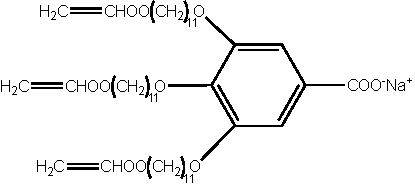
\includegraphics[width=\textwidth]{NaGA3C11.pdf}  %BJC: can color code this once I figure out how
              \vspace{0.05cm}
              \caption{}~\label{fig:monomer}
      \end{subfigure}
%      \begin{subfigure}{.3\textwidth}
%              \centering
%              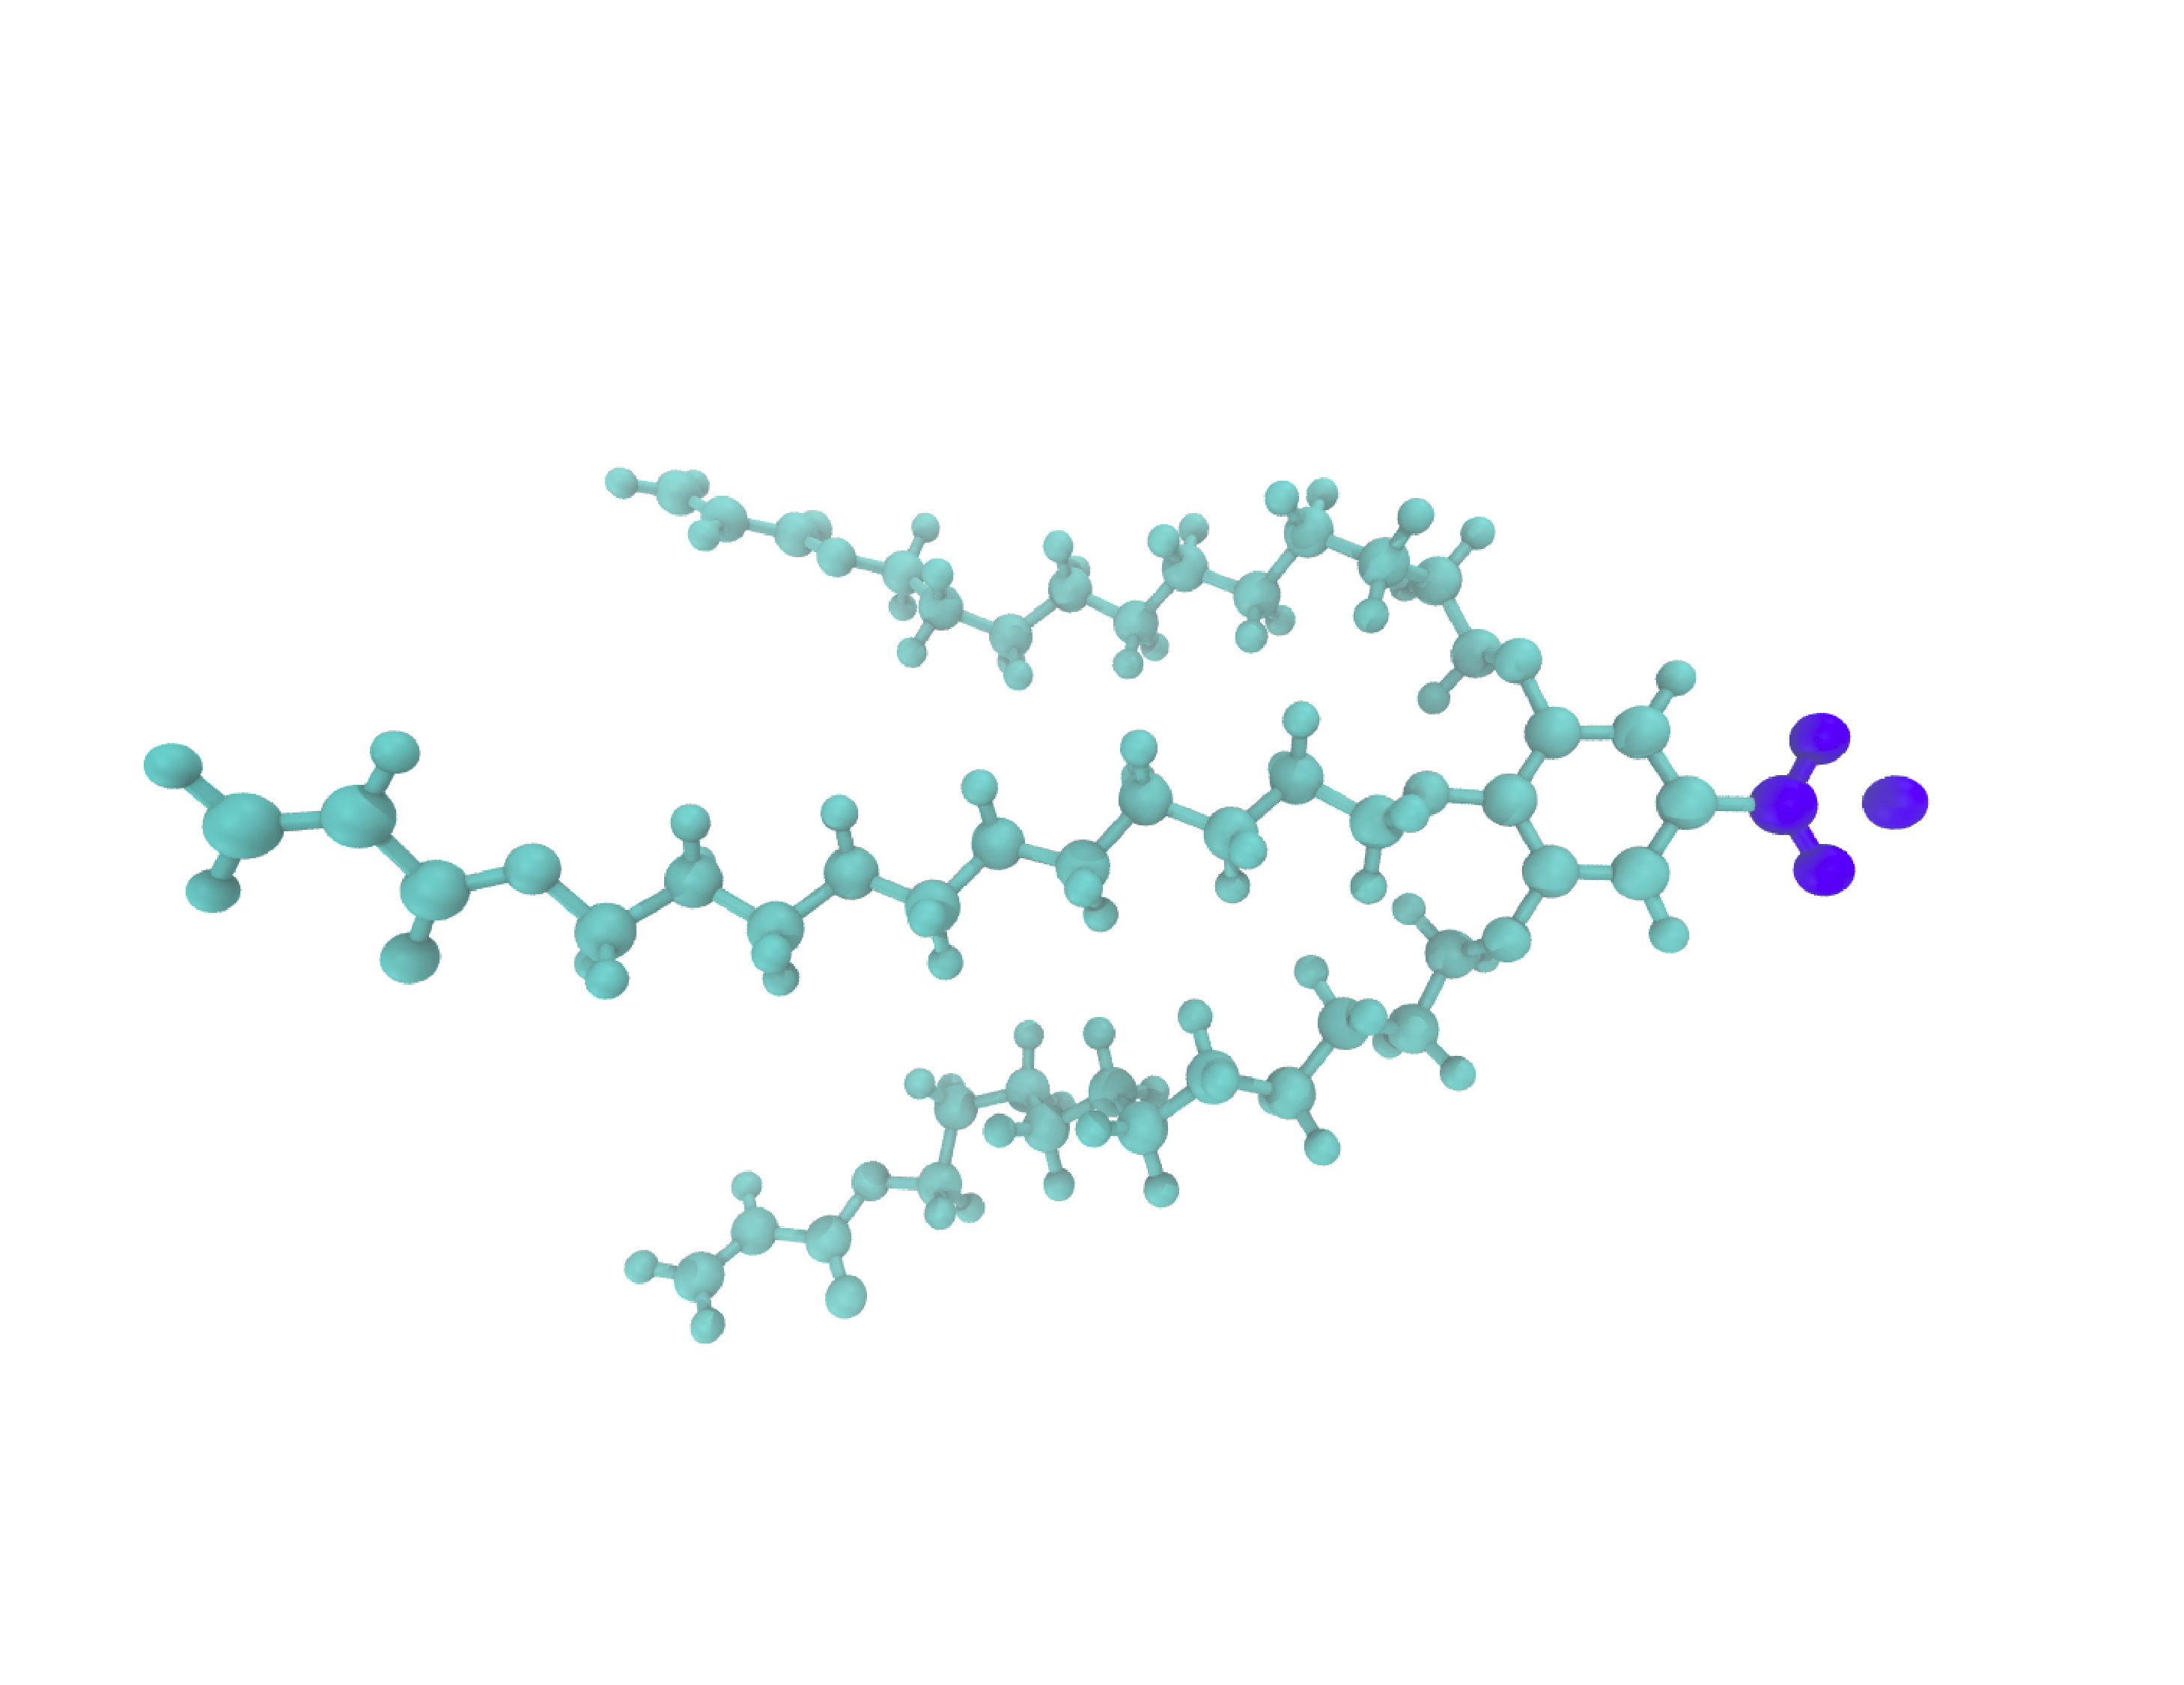
\includegraphics[width=\textwidth]{monomer_twocolor.pdf}
%              \caption{}~\label{fig:atomistic_monomer}
%      \end{subfigure}
%      \begin{subfigure}{0.3\linewidth}
%              \centering
%              
\includegraphics[width=0.6\textwidth]{wedge_thick.pdf}
%              \caption{}~\label{fig:wedge}
%      \end{subfigure}
              \begin{subfigure}{0.325\linewidth}
              \centering
              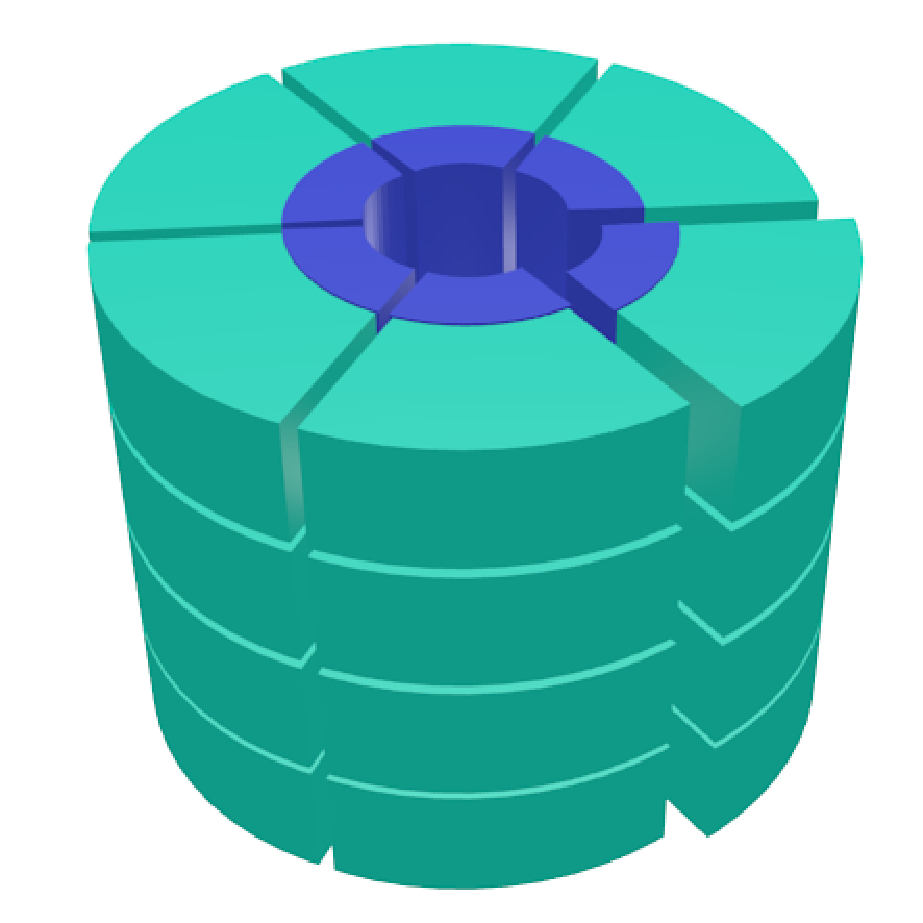
\includegraphics[width=0.6\textwidth]{columns.pdf}
              \caption{}~\label{fig:wedge_layer}
      \end{subfigure}
      \begin{subfigure}{0.325\linewidth}
              \centering
              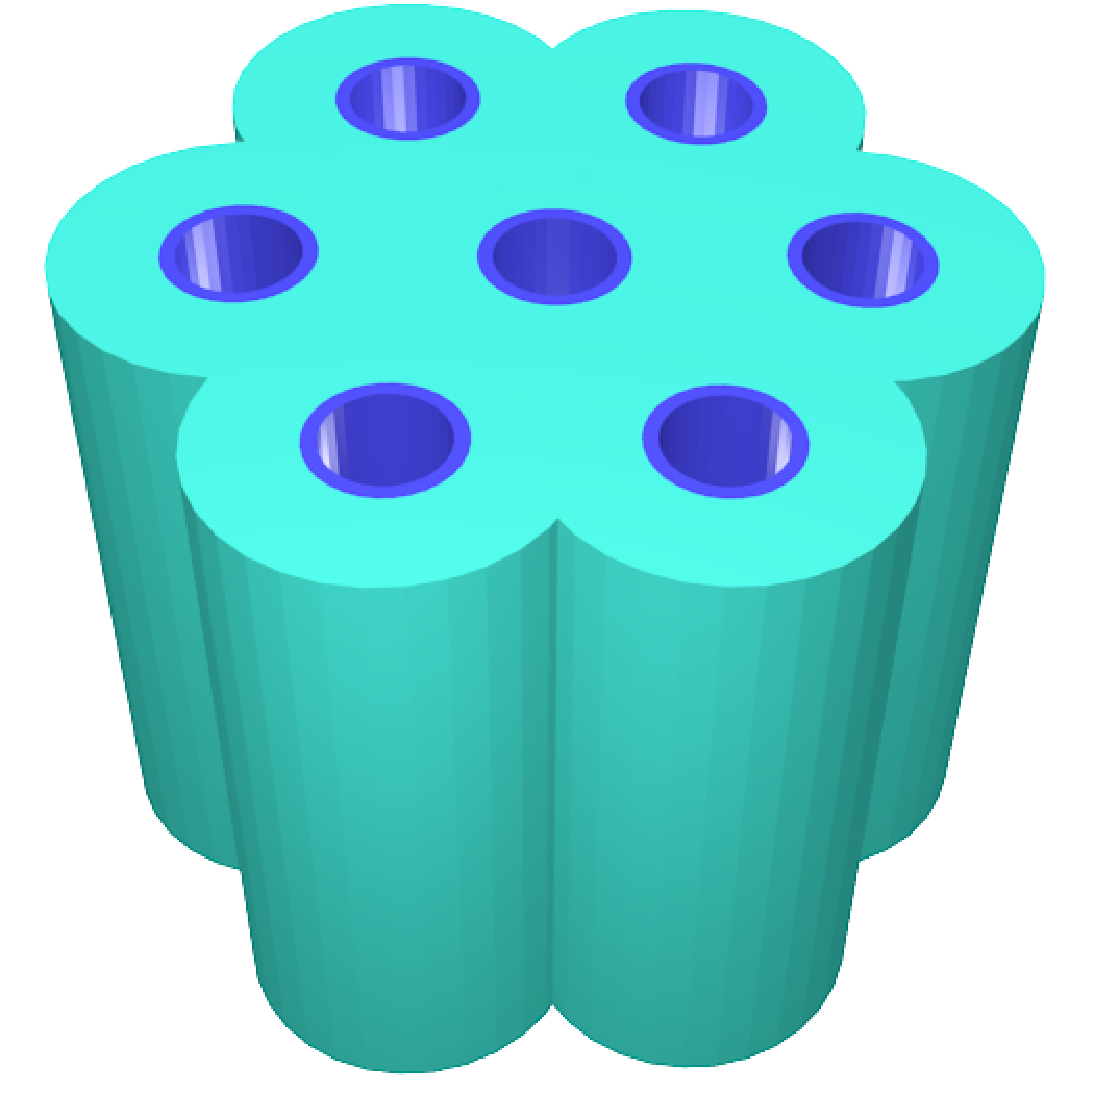
\includegraphics[width=0.6\textwidth]{hexagonal_packing.pdf}
              \caption{}~\label{fig:hex_packing_simple}
      \end{subfigure}
      \caption{(a) The LLC monomer Na-GA3C11 exhibits wedge-like character. (b) 
      Monomers stack on top of each other to create columns with short range order,
      then assemble into pores with hydrophilic head groups (blue) facing towards 
      the pore center. (c) The pores assemble into hexagonally packed columnar
      mesophases.}~\label{fig:assembly}
  \end{figure}
  
  \noindent We tested a number of different initial column architectures. 
  \begin{itemize}
      \item We stacked monomers in parallel displaced and sandwiched 
      configurations, two possible $\pi$-$\pi$ stacking modes.\cite{sinnokrot_estimates_2002}
      \item We also varied the initial distance between stacked monomers, $d$.
      \item We chose values of 3.7 \AA, based on experimental WAXS 
      measurements, as well as 5 \AA as a test of its sensitivity.
  \end{itemize}
  
  \noindent Our model's geometry is most consistent with experiment for systems
  built with 5 columns per pore and monomers initially stacked 3.7 \AA~apart
  (see Figure~\ref{fig:p2p}). 
  \begin{itemize}
    \item We equilibrated systems with 4, 5, 6, 7 and 8 columns per pore.
    \item The pore spacing of 5 column-per-pore systems agree well with experiment.
    \item 6 column-per-pore systems built with $d$ = 5 \AA~appear to yield an
    experimentally consistent pore spacing however, the equilibrated distance
    between stacked monomers stay close to 5 \AA~which is inconsistent with 
    experiment. 
    \item In general, the equilibrated distance between monomers stays close to
    its initial value. 
  \end{itemize}
  
  \begin{figure}[!htb]
    \centering
    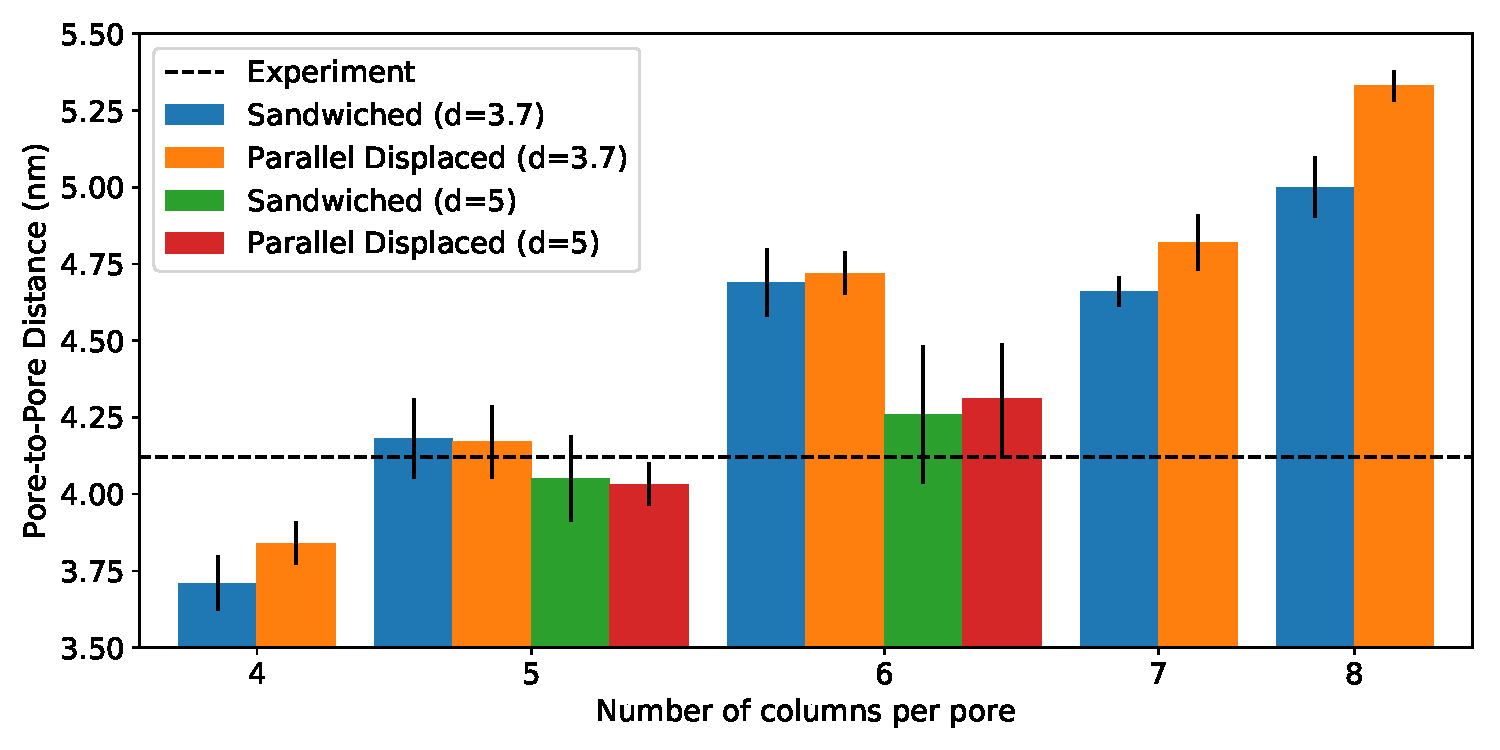
\includegraphics[width=\linewidth]{p2p.pdf}
    \caption{Systems with 5 columns per pore have equilibrated pore spacings
            closest to the experimental value of 4.12 nm. The equilibrated 
            pore spacing of the model increases as the number of columns in
            each pore increases.}~\label{fig:p2p}
  \end{figure}
  
%  \noindent On timescales that we can reasonably simulate, our equilibrated
%  structures show some initial configuration dependence. 
%  \begin{itemize}
%    \item All of the systems used to generate Figure~\ref{fig:p2p} are at 
%    least metastable.
%    \item We observe no large scale rearrangements that would be necessary
%    for all structures to converge to the same equilibrium structure. 
%  \end{itemize}

  \noindent We further validated the structure of our molecular model by 
  verifying its consistency with five major reflections present in the 
  experimental WAXS pattern.
  \begin{itemize}
    \item The five major reflections and the structural features leading
    to them are summarized and described in the caption of Figure~\ref{fig:WAXS_comparison}.
    \item Using MD trajectories, we simulated X-ray diffraction (XRD) 
    patterns that we could compare to the WAXS data by taking the 
    appropriate cross-section of the time-averaged 3D structure factor. 
    \item None of the models simulated to this point could reproduce R-double.   
  \end{itemize}   
  
  \noindent It is necessary to add a small amount of water to our model in
  order to fully reproduce all features of the WAXS pattern (see 
  Figure~\ref{fig:solvated_XRD}).
  \begin{itemize}
    \item We built our most experimentally consistent structure in the 
    parallel displaced configuration with 1 wt\% water added to the 
    pores. 
    \item This is the only configuration that gives rise to the 
    R-double feature. 
    \item R-double appears because vertically adjacent monomer head groups
    hydrogen bond with shared water molecules, causing them to be drawn 
    closer together.
    \item When multiple pairing interactions occur in series along the 
    same pore axis, the center of masses of the pairs are spaced apart at 
    twice the $\pi$-stacking distance. 
    \item The necessity of water in our model suggests that the membrane
    synthesized by Feng et al. was slightly hydrated due to water molecules
    leached from surroundings by the hydroscopic monomers. 
  \end{itemize}
  
  %\begin{wrapfigure}{L}{0.5\textwidth}
  \begin{figure}[!htb]
  	\centering
    \begin{subfigure}{0.49\linewidth}
    	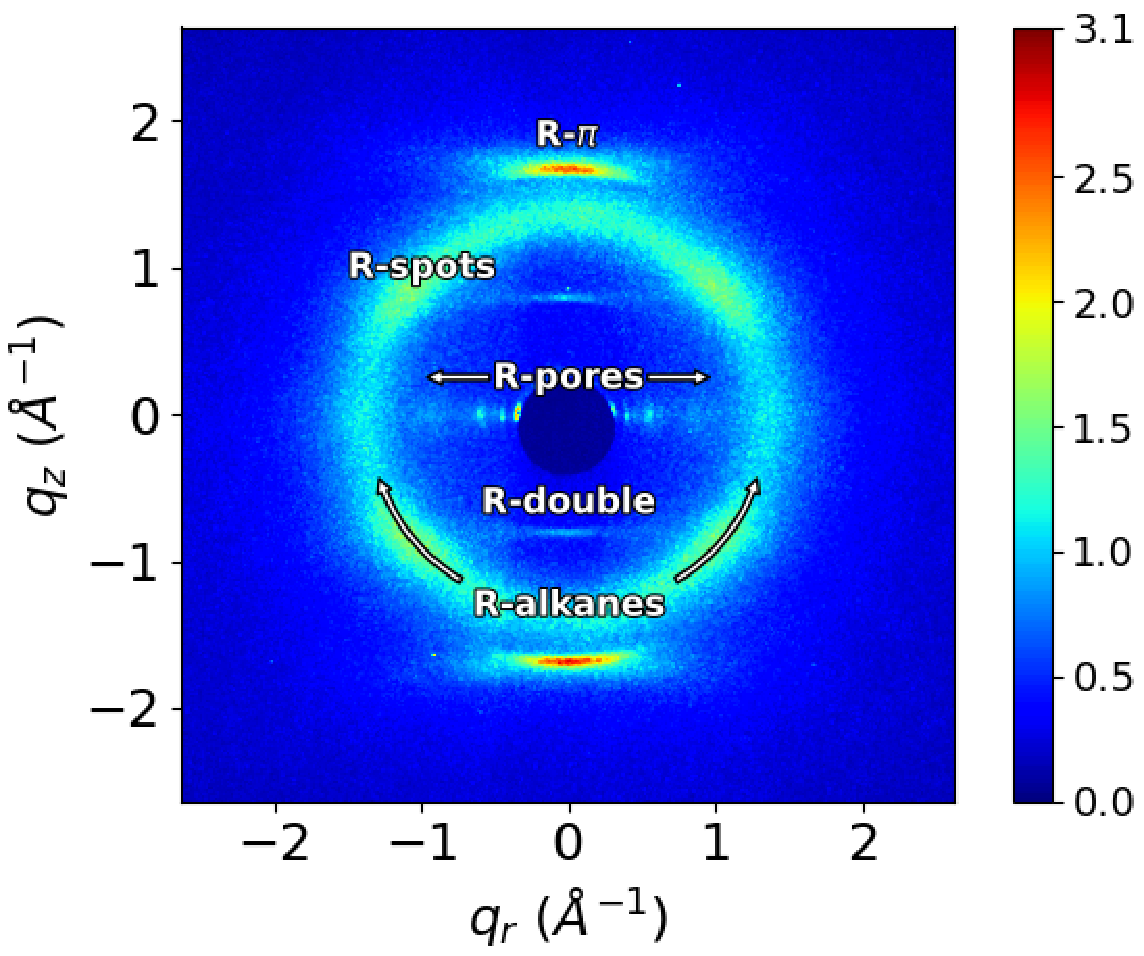
\includegraphics[width=\linewidth]{WAXS_annotated_words.pdf}
        \caption{Experiment}\label{fig:WAXS}
    \end{subfigure}
	\begin{subfigure}{0.49\linewidth}
        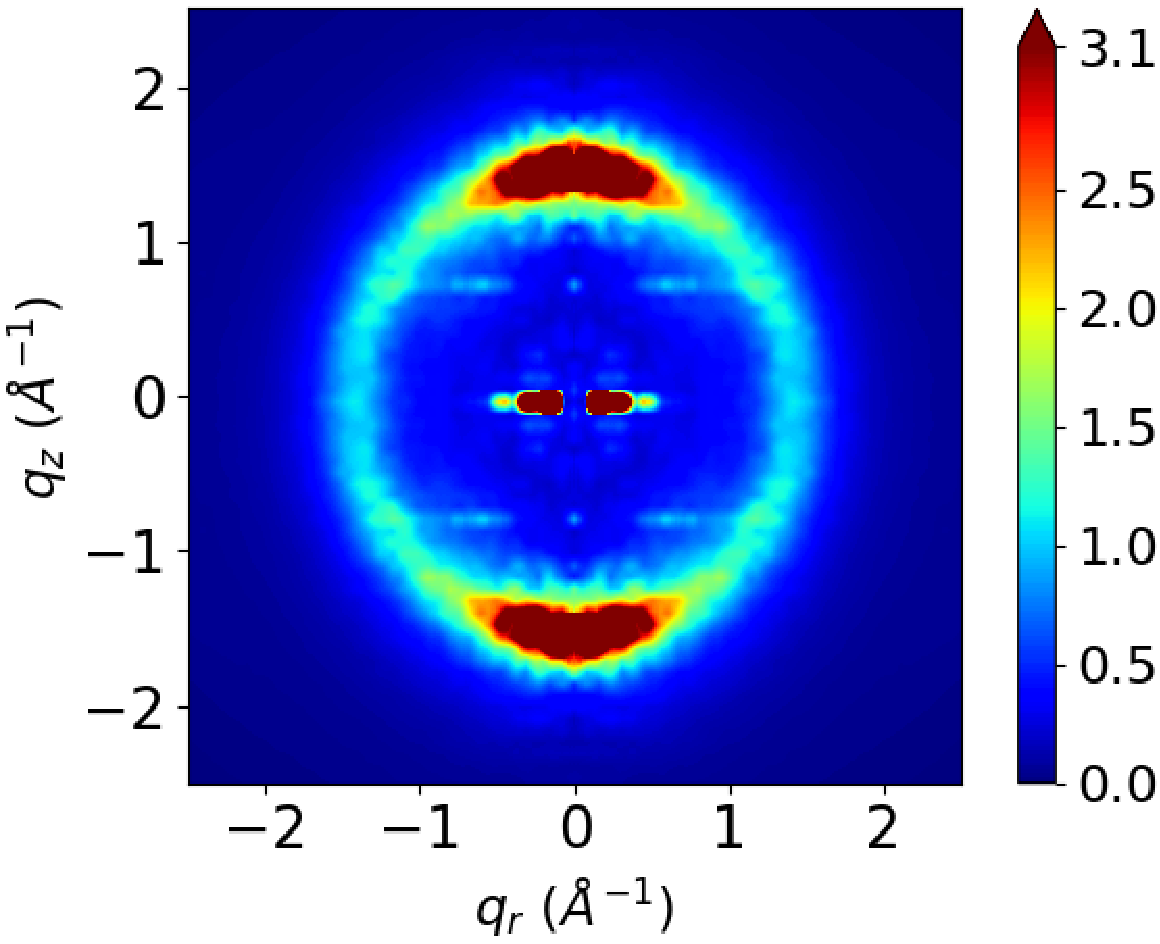
\includegraphics[width=\linewidth]{solvated_offset_rzplot_1.pdf}
        \caption{Simulation}\label{fig:solvated_XRD}   
	\end{subfigure}
    \caption{(a) 2D-WAXS gives details about repeating features on the order of
    angstroms. Our explanations for each of the 5 major reflections present are
    as follows: (R-$\pi$) Aromatic head groups $\pi-\pi$ stack 3.7 \AA~apart. 
    (R-double) Monomer head groups associate into pairs by hydrogen bonding with
    a shared water molecule. (R-alkanes) Alkane chain tails pack 4.5 \AA~apart. 
    (R-spots) Monomer tails pack hexagonally. (R-pores) The pores are spaced 
    4.12 nm apart and pack hexagonally. (b) We obtain a maximally consistent
    match between simulated XRD patterns and experimental WAXS data when we
    build systems in the parallel displaced configuration with 1 wt \% water
    included in the pores.}\label{fig:WAXS_comparison}
 \end{figure}
 %\end{wrapfigure}
 
  %BJC: I think this is important to say somewhere
  %BJC: but I don't have an ensemble of 1 wt % systems to fully prove that with.
  %BJC: I could show cross-sections of R-pi, but that would require more context. 
  \noindent On the timescales that we can reasonably simulate, our model
  exhibits slow dynamics. 
  \begin{itemize}
    \item Consequently, there are very few uncorrelated frames in our 
    trajectories which leads to noise in the simulated XRD patterns. 
    \item We can overcome this issue by combining the structure factors
    generated from an ensemble of trajectories produced starting from 
    an ensemble of uncorrelated initial configurations.
  \end{itemize}
 
  \noindent The composition of the pores does not change regardless of which
  initial configuration we study.
  \begin{itemize}
    \item In Figure~\ref{fig:overlaid_densities}, we plot the radial density
    of various monomer components as a function of distance from the pore
    centers. 
    \item All are qualitatively similar meaning that a solute placed in 
    any of these systems should experience a similar chemical environment.
    \item Although we will move forward with our most promising configuration,
    this is an important finding since it implies that we do not need to apply
    the same level of rigor when screening new monomers.
  \end{itemize}
  
  \begin{figure}[!htb]
  \centering
  \begin{subfigure}{\textwidth}
  %BJC: probably change this legend to `d = x Angstroms` instead of 
  % disordered/ordered, since I don't have space to talk about ordered / disorderd configurations (requires 
  % nematic order parameter to give a complete justification of the names)
  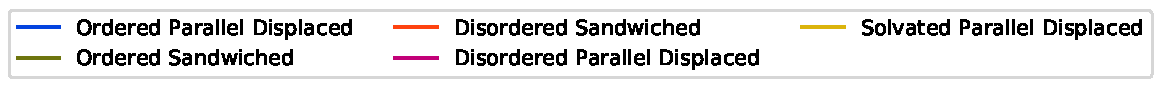
\includegraphics[width=\textwidth]{regional_density_legend.pdf}
  \end{subfigure}
  \begin{subfigure}{0.32\textwidth}
        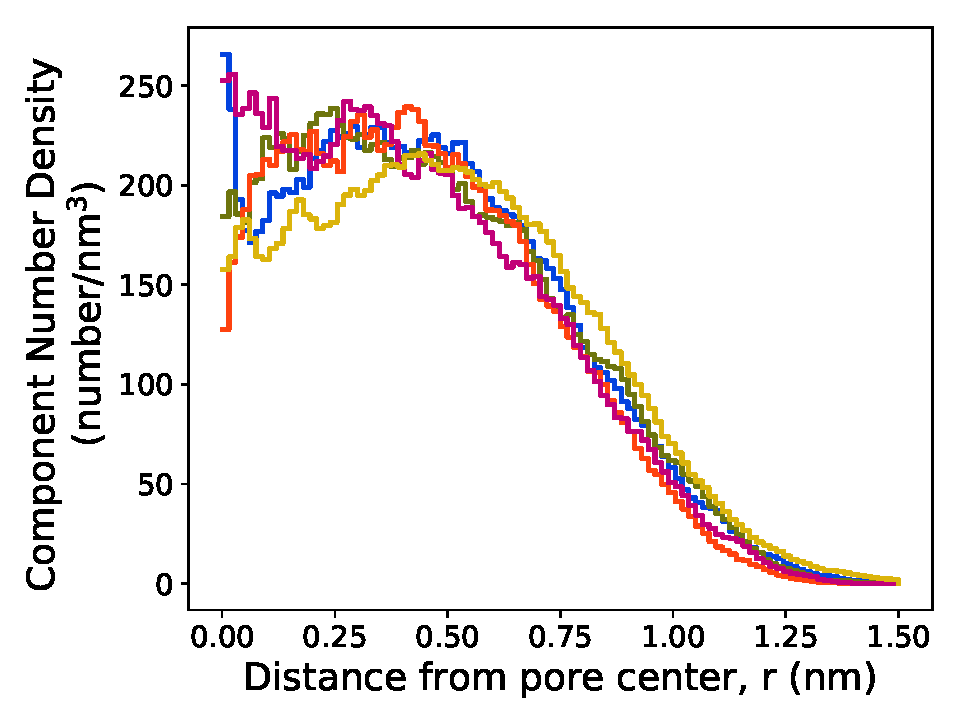
\includegraphics[width=1\linewidth]{head_group_density.pdf}
        \caption{Head Groups}
        \label{fig:head_groups_regional_density}
  \end{subfigure}
  \begin{subfigure}{0.32\textwidth}
        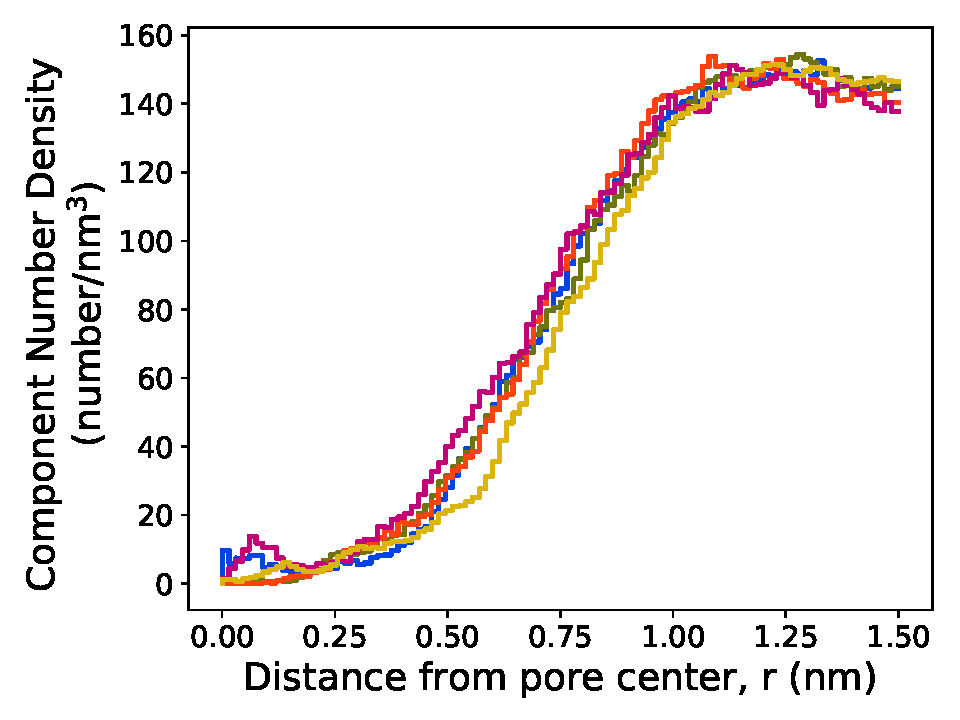
\includegraphics[width=1\linewidth]{tails_density.pdf}
        \caption{Tails}
        \label{fig:tails_regional_density}
  \end{subfigure}
  \begin{subfigure}{0.32\textwidth}
        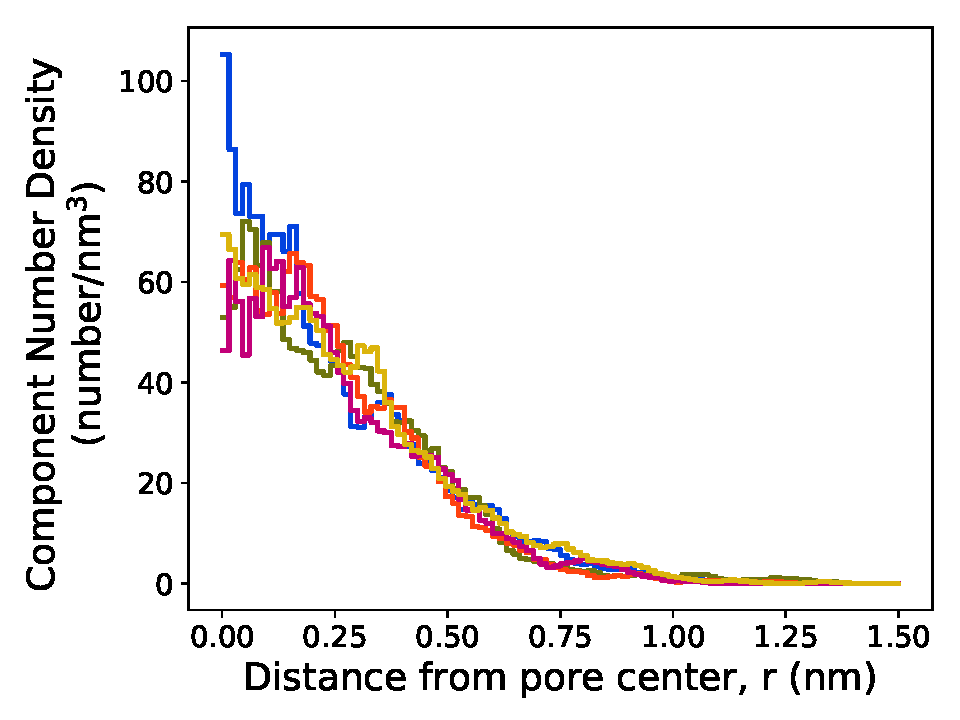
\includegraphics[width=1\linewidth]{sodium_density.pdf}
        \caption{Sodium Ions}
        \label{fig:sodium_regional_density}
  \end{subfigure}
  %MRS: not clear what is meant by ``all cases''
  \caption{In all cases, the component radial distribution functions are similar.
      They exhibit a composition gradient transitioning from the hydrophilic to the hydrophobic
          regions. The biggest differences are at r=0 where noise is higher due to
          decreased sampling. The center of the pore is not hollow, but contains sodium ions and
          head groups, even when the system is solvated. This architecture may impede transport in
          the real system in a chemically-dependent manner.
          The solvated system has a lower density of head groups near the
          pore center which is likely due to the swelling that is necessary in order to fit water
          molecules in the pore region.}~\label{fig:overlaid_densities}
  \end{figure}
  
  \noindent \textbf{\large Objective 2:} \textit{\large Determine transport mechanisms} (\textcolor{green!40!olive}{\textbf{Complete}})
  
  \noindent We added additional water to our most experimentally consistent
  structural model in order to create a higher water content H\textsubscript{II}
  phase model.
  \begin{itemize}
    \item There have been a range of reported water contents used to 
    form the H\textsubscript{II} phase with this particular monomer.
    \item Although Resel et al. commented that the system is likely
    already fully hydrated at 7 wt \% water with additional water
    trapped in defects between mesophases.\cite{resel_structural_2000}
    \item Therefore, we built two systems with 5 and 10 wt\% water.
  \end{itemize}
  
  \noindent We observed that water partitions into the distal tail region.
  \begin{itemize}
    \item We define the distal tail region to be any radial distance 
    greater than 1.5 nm from any pore center. 
    \item There is approximately a 3:2 ratio of water in the pores to
    water in the distal tails. 
    \item Due to the wedge shape of the monomers, the distal tail region
    has a relatively low density leaving space for water molecules to 
    fill.  
  \end{itemize}
  
  \noindent The pores of the H\textsubscript{II} phase are primarily a 
  mixture of water and sodium ions.
  \begin{itemize}
    \item The maximum density of head groups occurs 0.45 and 0.65 nm from
    the pore center in the 5 and 10 wt\% water systems respectively (see
    Figure~\ref{fig:component_densities}). 
    \item There are almost no head groups occupying the pore center.
  \end{itemize}
  
  \begin{figure}[!htb]
  \centering
  \begin{subfigure}{0.45\textwidth}
  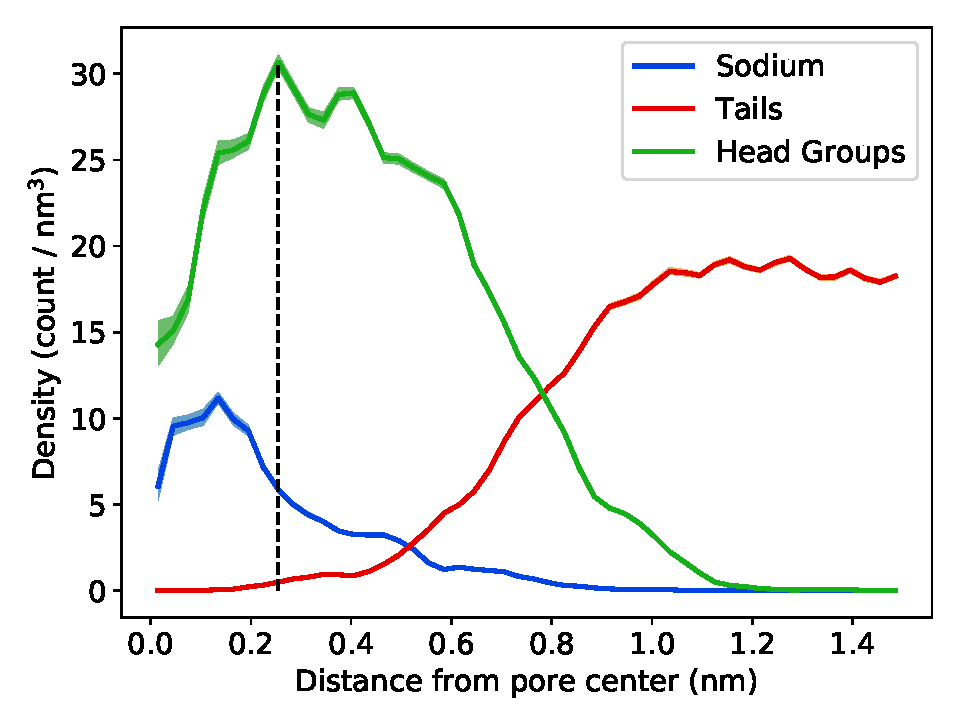
\includegraphics[width=\textwidth]{component_density_dry.pdf}
  %BJC: simulation is extended to smooth out these curves
  \caption{Dry System}\label{fig:component_density_dry}
  \end{subfigure}
  \begin{subfigure}{0.45\textwidth}
  \vspace{-0.5cm}
  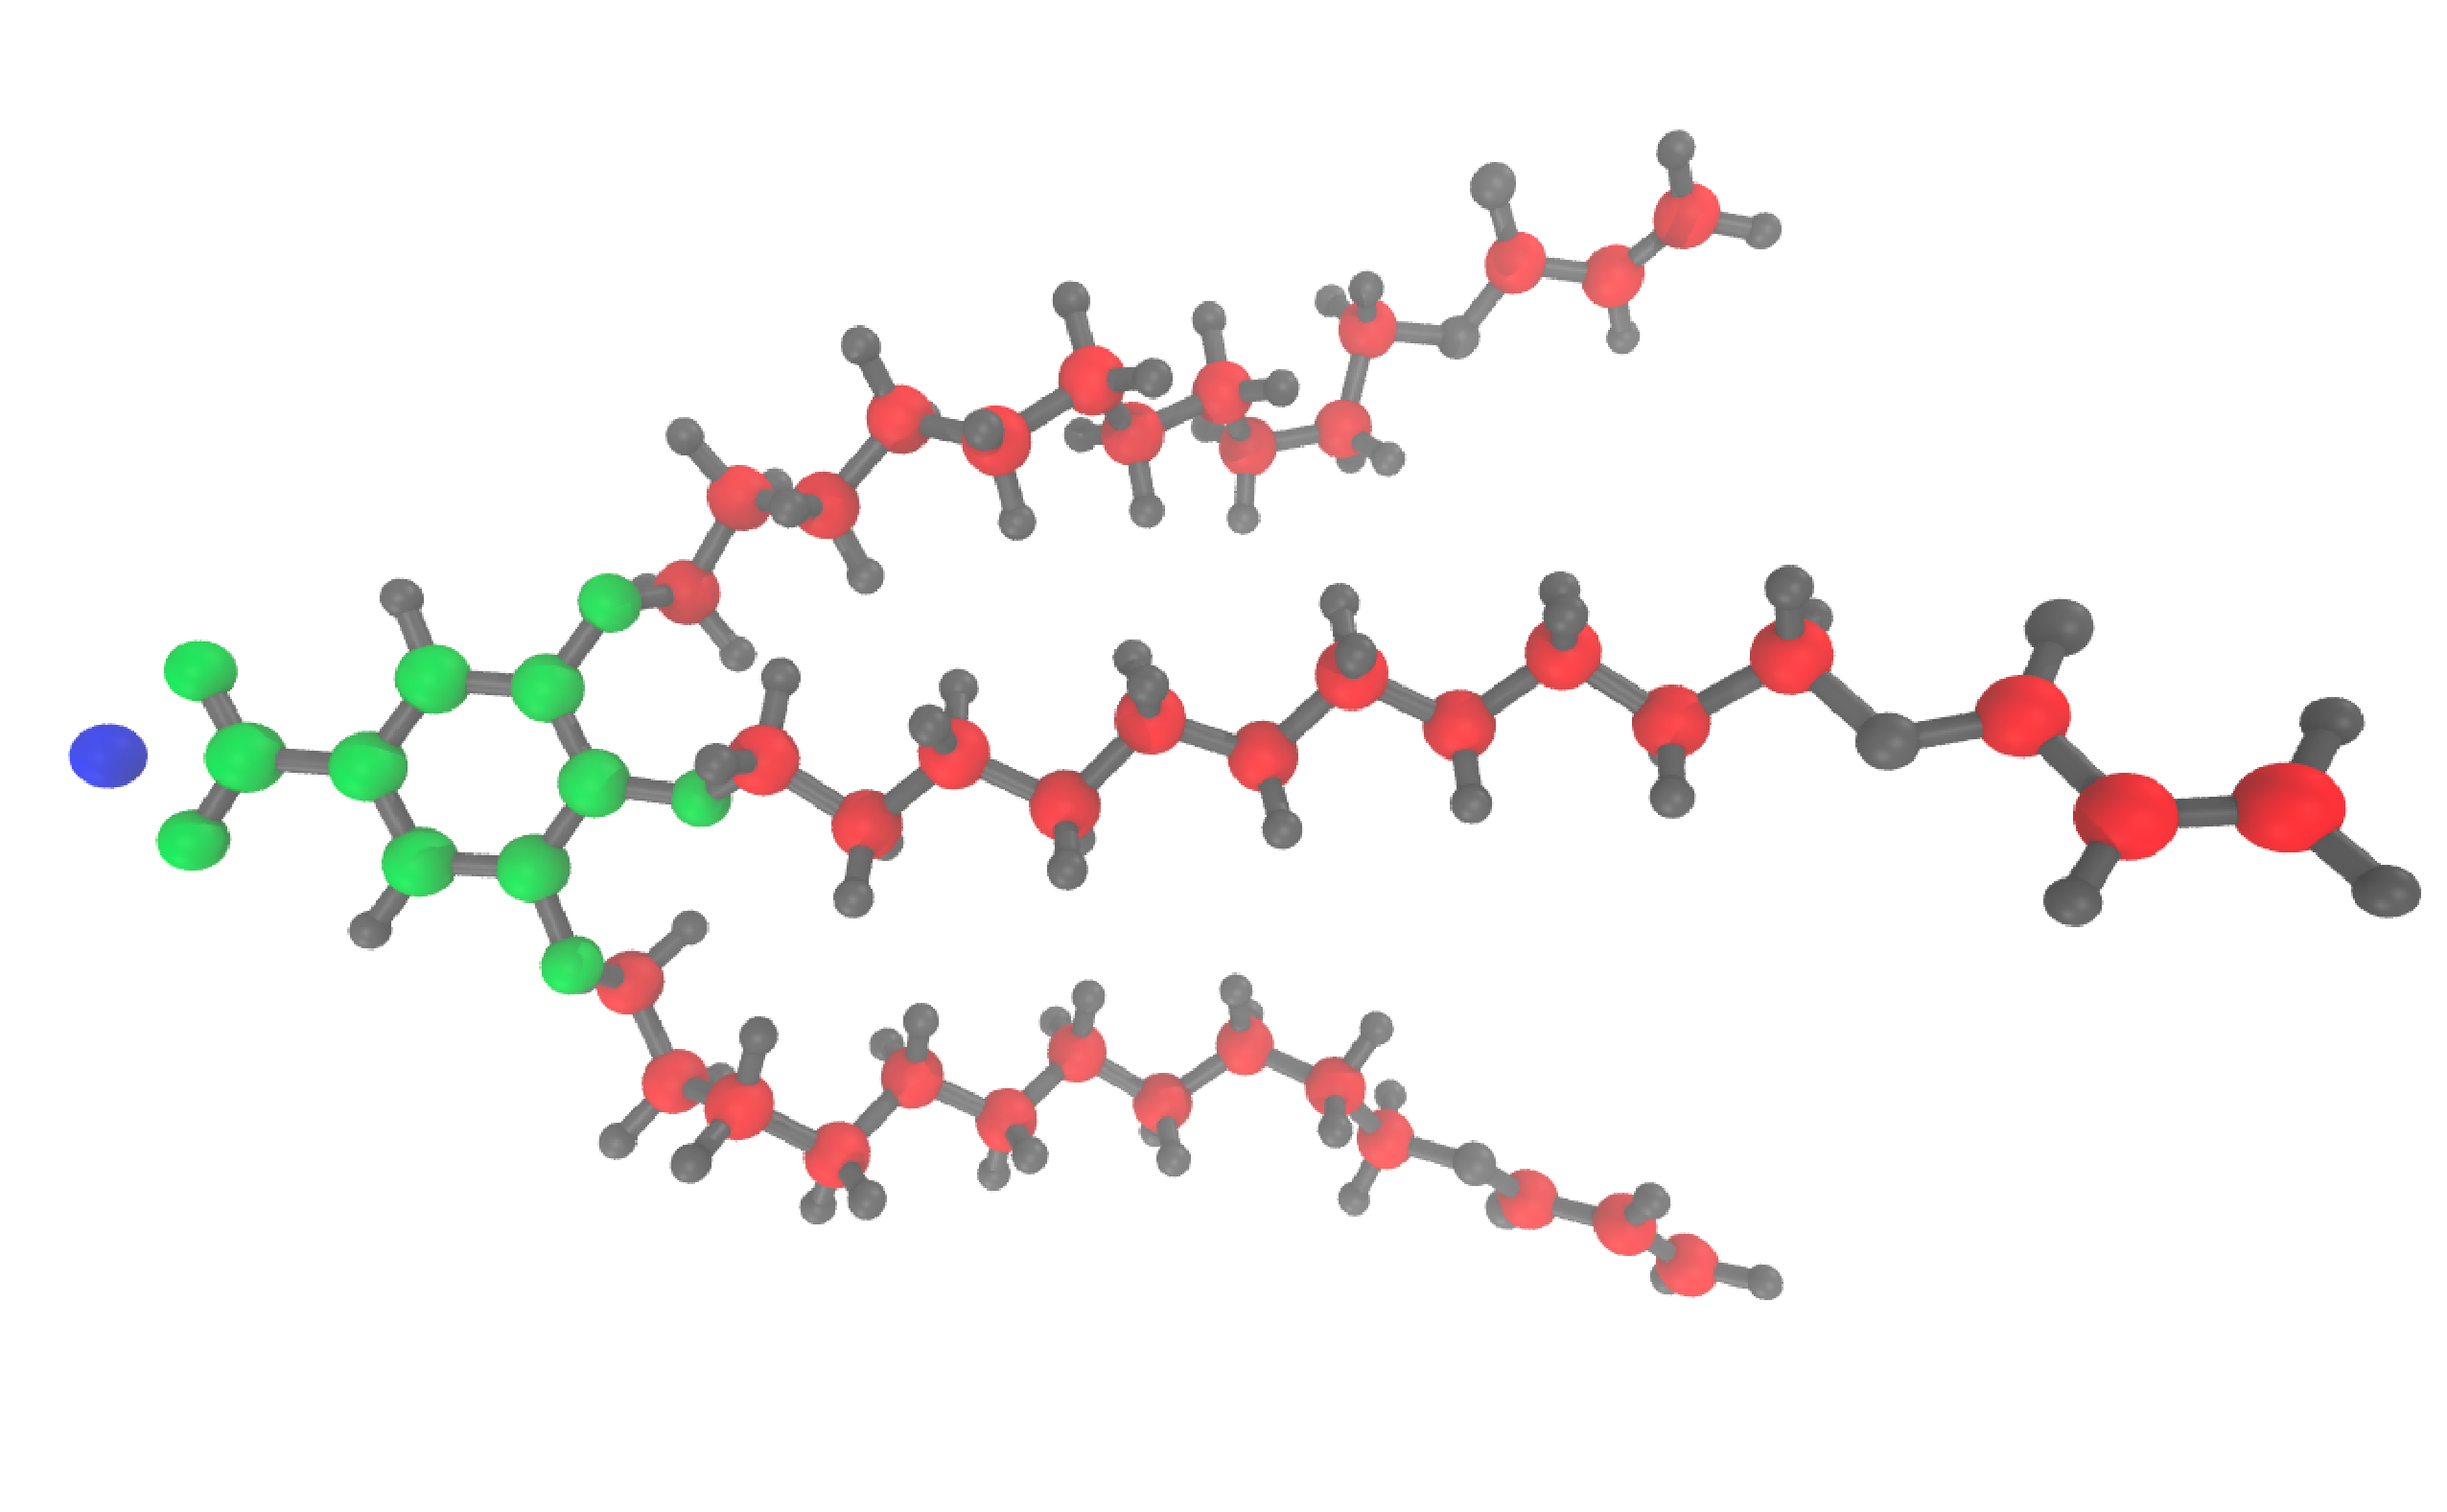
\includegraphics[width=\textwidth]{monomer_color_coded.pdf}
  \label{fig:monomer_color_coded}
  \end{subfigure}
  \begin{subfigure}{0.45\textwidth}
  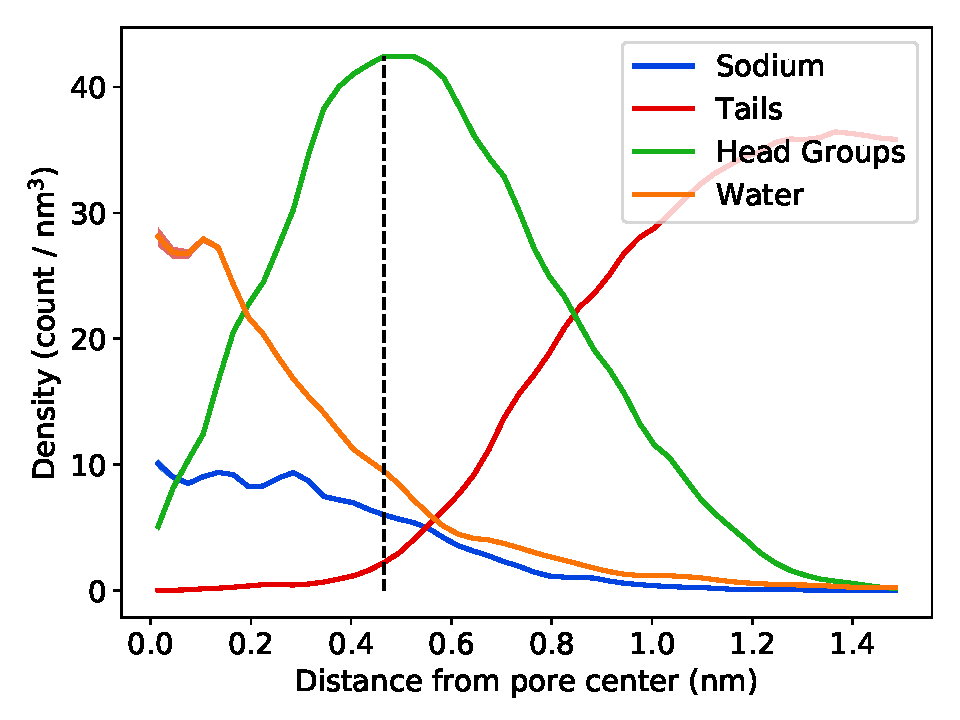
\includegraphics[width=\textwidth]{component_density_5wt.pdf}
  \caption{5 wt\% water}\label{fig:component_density_5wt}
  \end{subfigure}
  \begin{subfigure}{0.45\textwidth}
  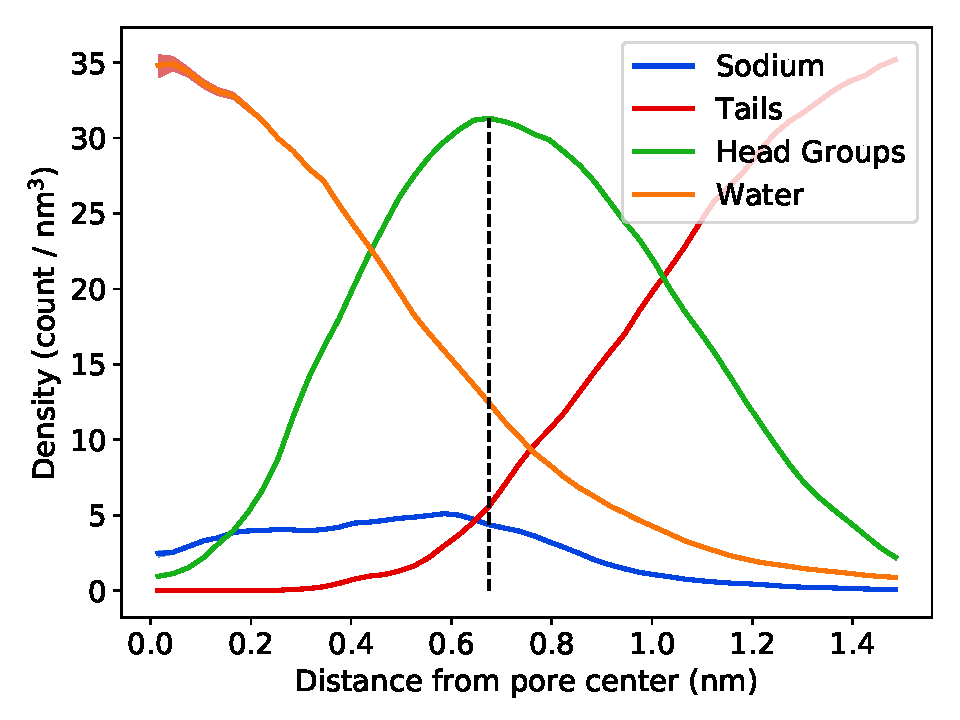
\includegraphics[width=\textwidth]{component_density_10wt.pdf}
  \caption{10 wt\% water}\label{fig:component_density_10wt}
  \end{subfigure}
  \caption{The radial densities of various monomer components paint a
  picture of the pore topology where the pore centers are primarily composed
  of water and sodium ions. The monomer groups labeled in each plot correspond to
  the color-coded monomer pictured in the upper right corner of the figure.
  All RDFs represent the number of atoms located at a given distance from the
  pore center normalized by the volume of the annular bin to which they belong.
  (a) In the dry system, the density of head groups and sodium ions are highest
  within 0.25 nm of the pore center. (b) In the 5 wt \% system, monomer head
  groups retreat about 0.2 nm radially in order to make room for water molecules.
  (c) Monomers in the 10 wt \% system retreat an additional 0.2 nm to make room
  for more water.}\label{fig:component_densities}
  \end{figure}
  
  \noindent Water and sodium transport is significantly faster in the less
  crowded 10 wt\% water pores. 
  \begin{itemize}
    \item The mean squared displacement (MSD) of water is about 51 times 
    higher and the MSD of sodium is about 49 times higher compared to the 5 wt\% system.
    \item In general we observe similar solute transport mechanisms in the 5
    and 10 wt\% water systems but on different time scales.
    %BJC: might as well leave 5 wt% data in there.
%    \item Therefore, we focus the remainder of this discussion on the 10 wt\%
%    water system since we were able to collect a larger quantity of mechanistic
%    data from the solute trajectories.
  \end{itemize}
  
  % BJC: do you think I can get away with an appendix with the solute table + abbreviations that
  % doesn't count towards the page limit?
  \noindent We observed transport of 20 different small polar solutes in the
  pores of our model. 
  \begin{itemize}
    \item We created a separate initial configuration for each solute studied and
    placed 6 solutes, equally spaced in $z$, in each nanopore.
    \item After a brief equilibration, we allowed the solutes to simulate for
    1 microsecond. 
  \end{itemize}
  
  \noindent The solute MSDs are not a monotonic function of solute size.
  \begin{itemize}
    %MRS: Talk about data presentations (figures) in the present tense.  
    \item In Figure~\ref{fig:all_msds_10wt}, we plotted the average
    MSD of each solute. 
    \item In Figure~\ref{fig:msd_radius_10wt}, we plotted solute
    MSDs against their molecular radius.
    \item We also plotted theoretical curves which illustrate the 
    expected MSD of each solute if they were to travel unhindered.
    \item We ensured that the Stokes-Einstein equation with the
    correction factor of Gierer and Wirtz\cite{gierer_molekulare_1953}
    passed through methanol in order to give an approximate frame of reference. 
    \item Methanol is small and therefore can travel relatively
    unhindered compared to all other solutes.
    \item The correction factor attempts to include the effects of
    microfriction that begin to play a role when solute size becomes
    on the order of solvent size.
    \item The theoretical line can be used as an approximate boundary
    between subdiffusive, Brownian and superdiffusive behavior.
  \end{itemize}
  
  \begin{figure}[!htb]
  \centering
  \begin{subfigure}{0.45\textwidth}
  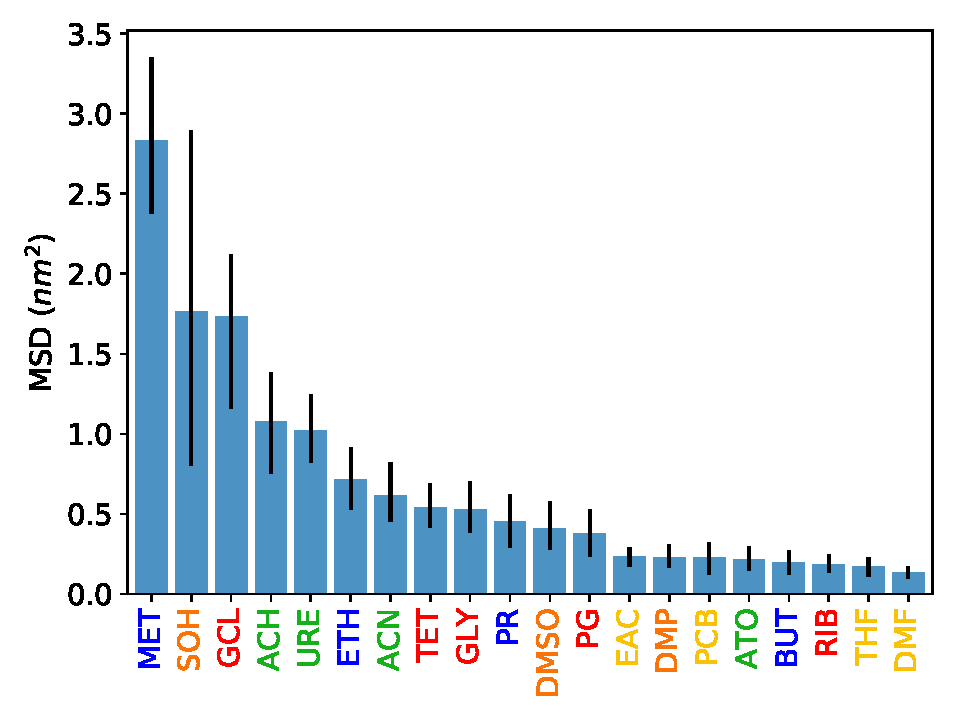
\includegraphics[width=\textwidth]{all_10wt_tamsds.pdf}
  \caption{10 wt \% water}\label{fig:all_msds_10wt}
  \end{subfigure}
  \begin{subfigure}{0.45\textwidth}
  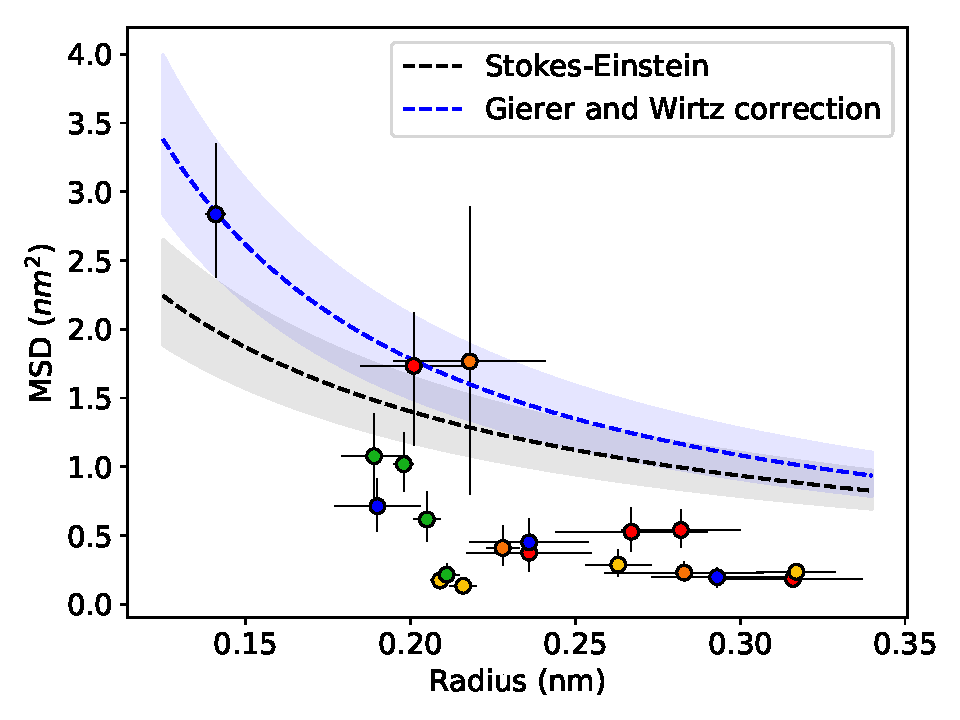
\includegraphics[width=\textwidth]{msd_radius_10wt.pdf}
  \caption{10 wt \% water}\label{fig:msd_radius_10wt}
  \end{subfigure}
  \caption{The MSDs of solutes in the 5 wt \% water system (a) are significantly
  smaller than those of the solutes in the 10 wt \% water system (b). The
  MSDs are not a monotonic function of molecular size (c and d). A significant
  number of solute MSDs fall below the theoretical lines predicted by the
  Stokes-Einstein equation and Gierer and Wirtz' corrected Stokes-Einstein equation.
  }\label{fig:msds}
  \end{figure}
  
% 5 and 10 wt %
%  \begin{figure}[!htb]
%  \centering
%  \begin{subfigure}{0.45\textwidth}
%  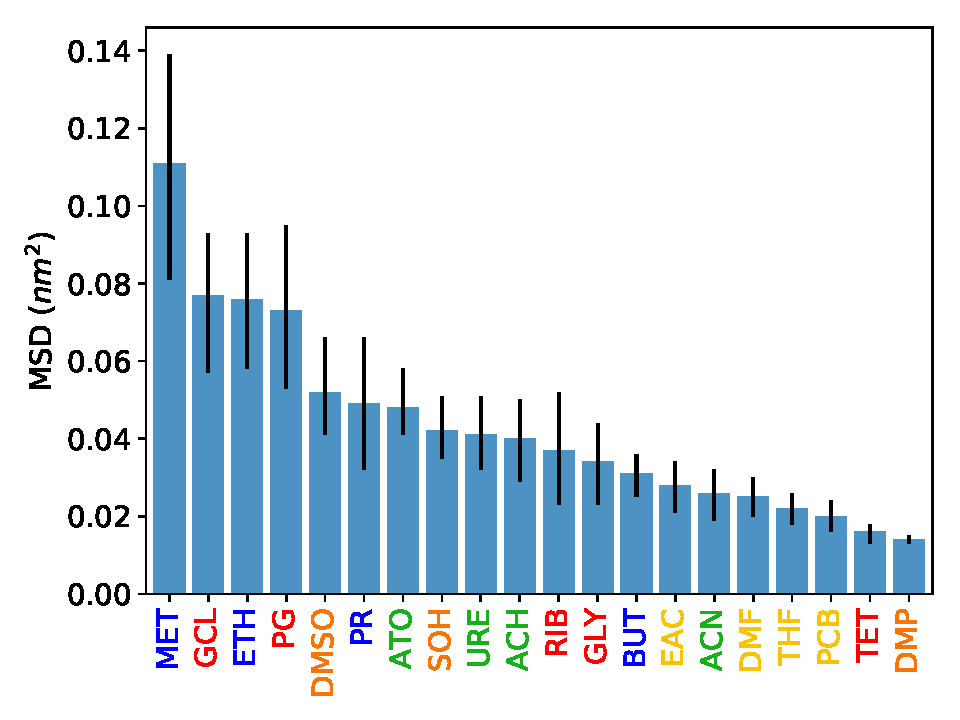
\includegraphics[width=\textwidth]{all_5wt_tamsds.pdf}
%  \caption{5 wt \% water}\label{fig:all_msds_5wt}
%  \end{subfigure}
%  \begin{subfigure}{0.45\textwidth}
%  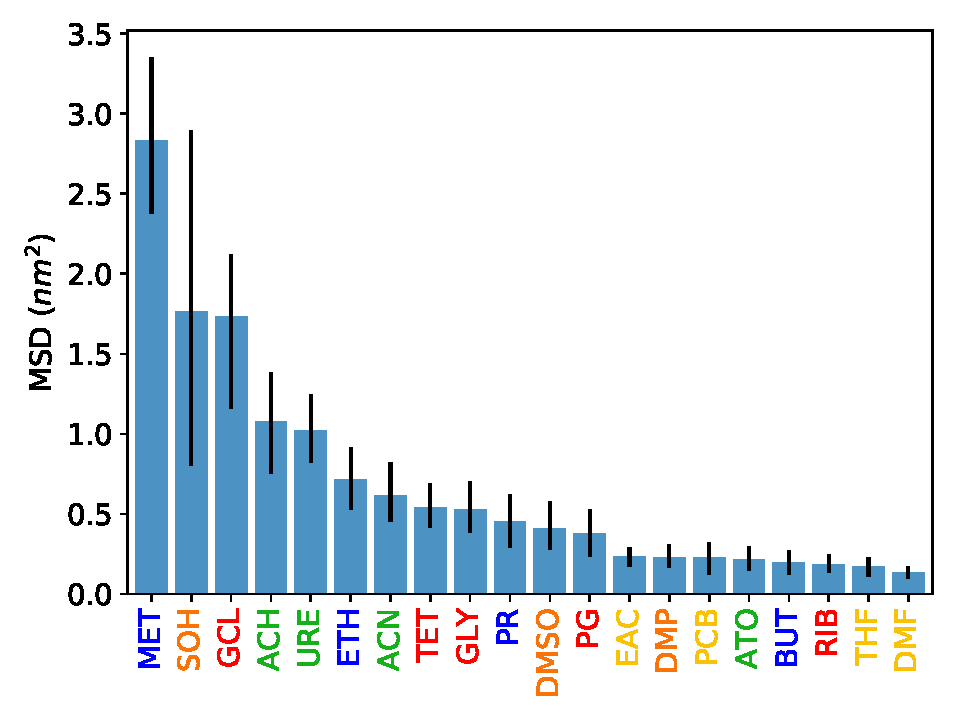
\includegraphics[width=\textwidth]{all_10wt_tamsds.pdf}
%  \caption{10 wt \% water}\label{fig:all_msds_10wt}
%  \end{subfigure}
%  \begin{subfigure}{0.45\textwidth}
%  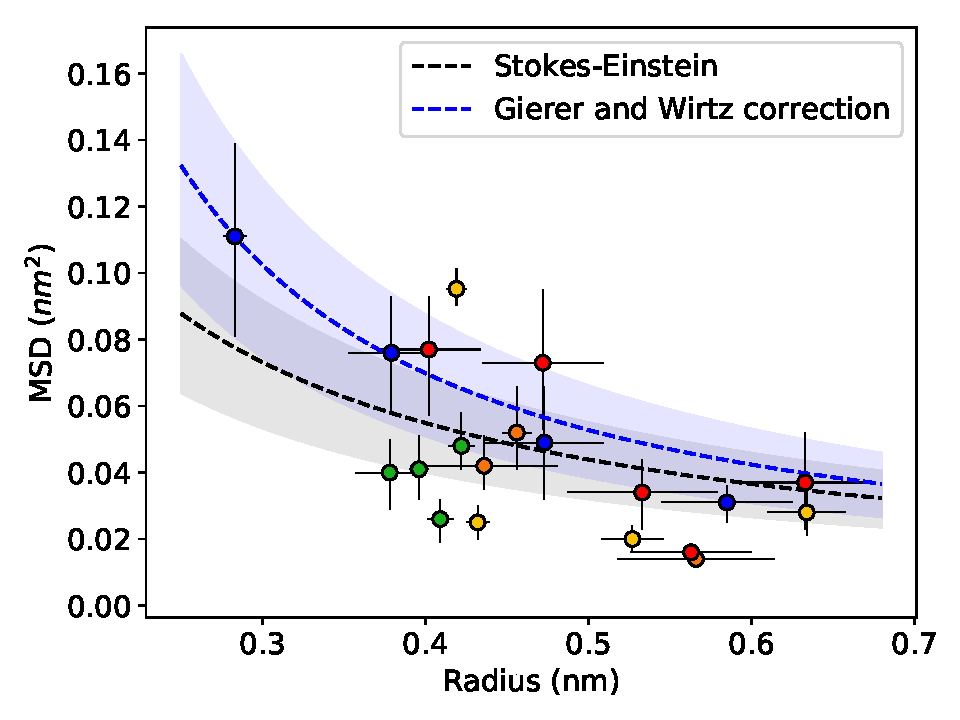
\includegraphics[width=\textwidth]{msd_radius_5wt.pdf}
%  \caption{5 wt \% water}\label{fig:msd_radius_5wt}
%  \end{subfigure}
%  \begin{subfigure}{0.45\textwidth}
%  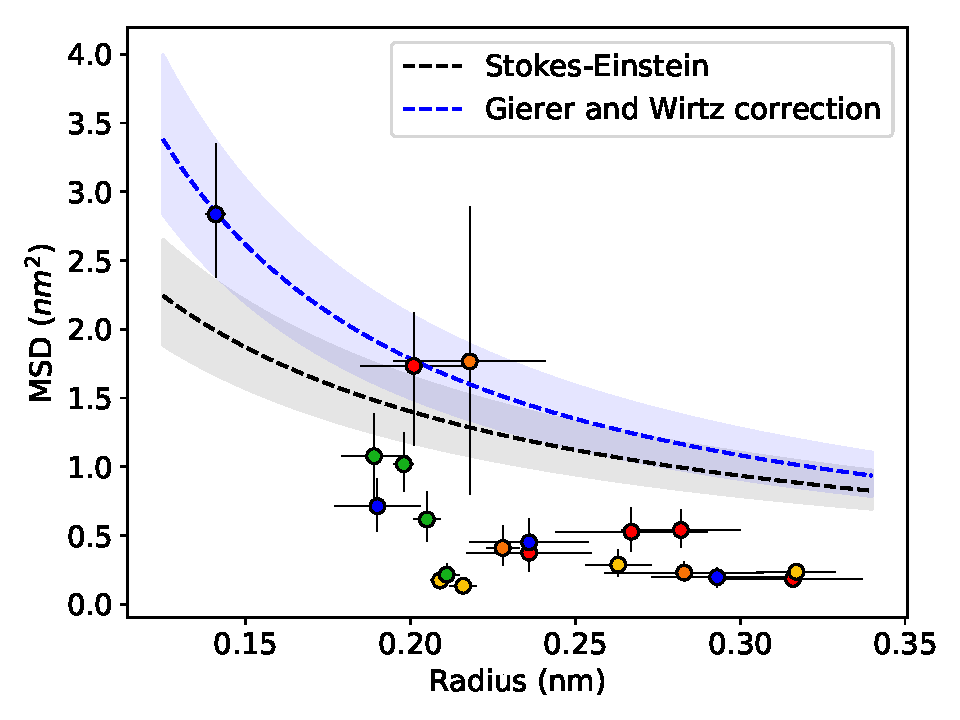
\includegraphics[width=\textwidth]{msd_radius_10wt.pdf}
%  \caption{10 wt \% water}\label{fig:msd_radius_10wt}
%  \end{subfigure}
%  \caption{The MSDs of solutes in the 5 wt \% water system (a) are significantly
%  smaller than those of the solutes in the 10 wt \% water system (b). The
%  MSDs are not a monotonic function of molecular size (c and d). A significant
%  number of solute MSDs fall below the theoretical lines predicted by the
%  Stokes-Einstein equation and Gierer and Wirtz' corrected Stokes-Einstein equation.
%  }\label{fig:msds}
%  \end{figure}
  
  \noindent Intermittent hops between long periods of entrapment lead
  to subdiffusive solute transport behavior. 
  \begin{itemize}
    \item As Figure~\ref{fig:msd_radius_10wt} implies, most solutes
    move significantly slower than expected.
    \item In Figure~\ref{fig:example_ztraces}, we've plotted the $z$-direction
    trajectory of three ethanol molecules.
    \item Typically, long periods of entrapment occur when ethanol 
    molecules are far from the pore center, while there is a much 
    greater degree of mobility close to the pore center.
    \item The MSD curve averaged over all ethanol trajectories is shown
    in Figure~\ref{fig:example_msd}.
    \item The curve is sub-linear and thus subdiffusive.
  \end{itemize}
  
  \begin{figure}[!htb]
  \centering
  \begin{subfigure}{0.49\textwidth}
  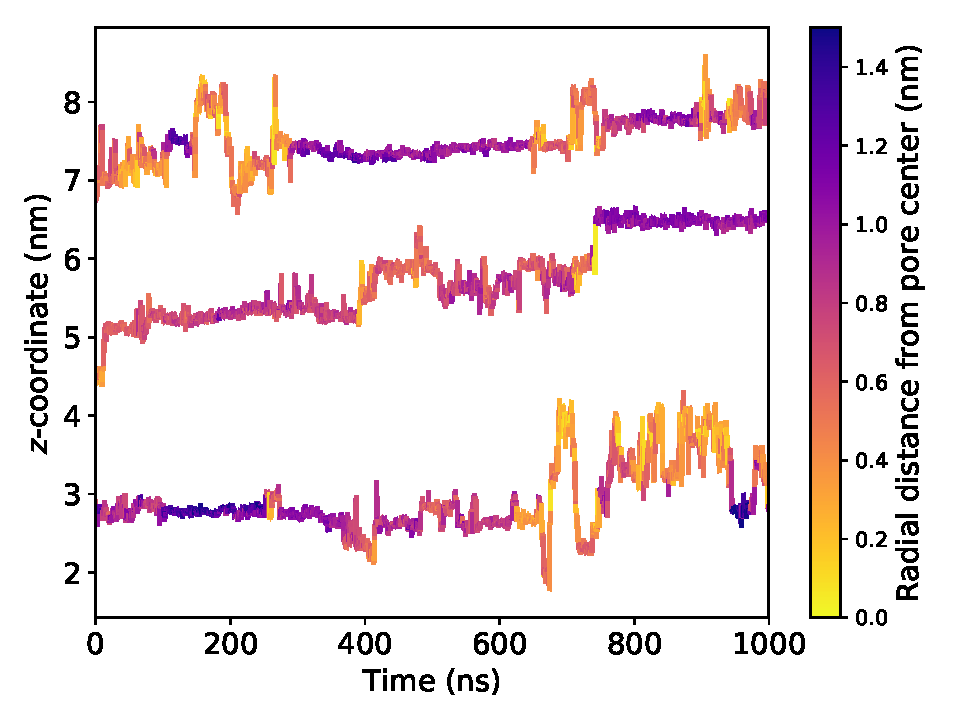
\includegraphics[width=\linewidth]{colorful_example_ztraces.pdf}
  \caption{}\label{fig:example_ztraces}
  \end{subfigure}
  \begin{subfigure}{0.49\textwidth}
  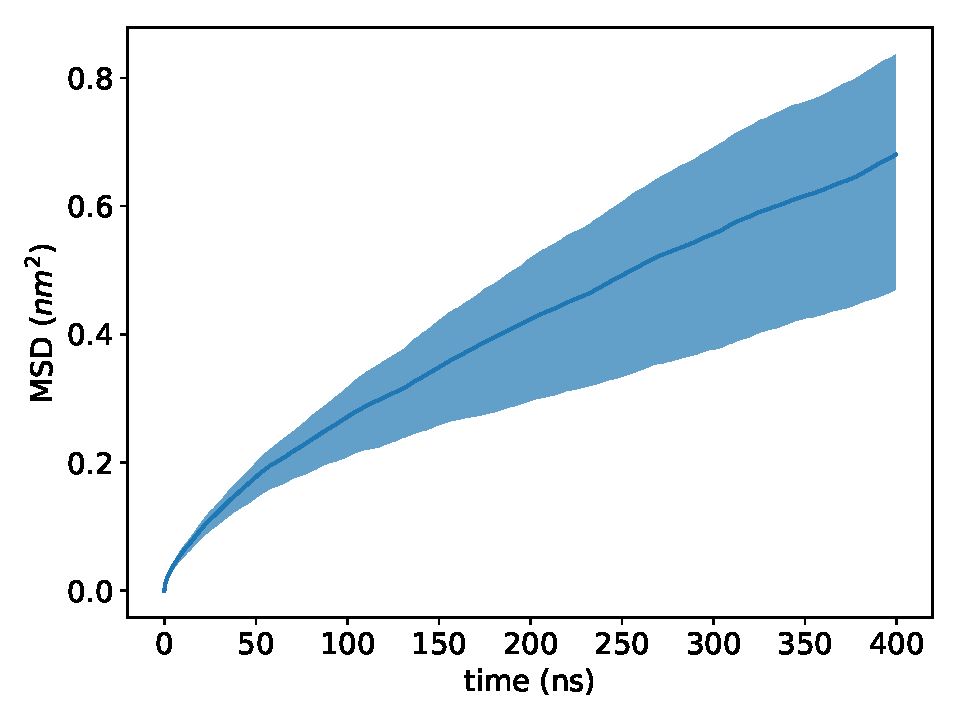
\includegraphics[width=\linewidth]{example_msd.pdf}
  \caption{}\label{fig:example_msd}
  \end{subfigure}
  \caption{All solutes show subdiffusive transport behavior inside the membrane's
  nanopores, similar to that exhibited by ethanol. (a) The $z$-coordinate trace of
  3 representative ethanol COMs shows clear periods of entrapment separated by hops.
  In general, the longest dwell times occur when solutes are situated far from the
  pore center and the hops occur when solutes are close to the pore center. (b) The
  time-averaged MSD of ethanol is sub-linear which suggests transport is governed
  by an anomalous subdiffusion process.}\label{fig:qualitative_mechanisms}
  \end{figure}
  
  \noindent We observe three mechanisms of entrapment that are responsible for 
  subdiffusive behavior.
  \begin{enumerate}
    \item As already demonstrated in Figure~\ref{fig:example_ztraces}, solutes that
    drift away from the pore center can become entangled in the monomer tails. 
    \item Many of the solutes we studied are capable of donating hydrogen bonds to
    monomer head groups and thus are prone to temporary immobilization through this interaction.
    \item Because all solutes are polar, they have regions of concentrated electron
    density, modeled as partial charges, which can associate with sodium ions
    partially bound to monomer head groups.
  \end{enumerate}
  
  Due to the crowded environment among the monomer tails, solutes generally move faster
  in the less dense pore region.
  \begin{itemize}
    \item Figure~\ref{fig:hop_lengths} shows that this is the case for all solutes.
    \item Hops made in the pore region are on average 59 \% larger than those made
    outside the pore region.
  \end{itemize}
  
  However, time spent in the pore region does not necessarily result
  in a high MSD. 
  \begin{itemize}
    \item For example, ribose spends the largest fraction of time in 
    the pore region, but has the fifth lowest hop frequency and the third 
    lowest average MSD (see Figures~\ref{fig:frac_time} and ~\ref{fig:hopfreq}).
  \end{itemize}
  
  \begin{figure}
  \centering
  \begin{subfigure}{0.325\textwidth}
  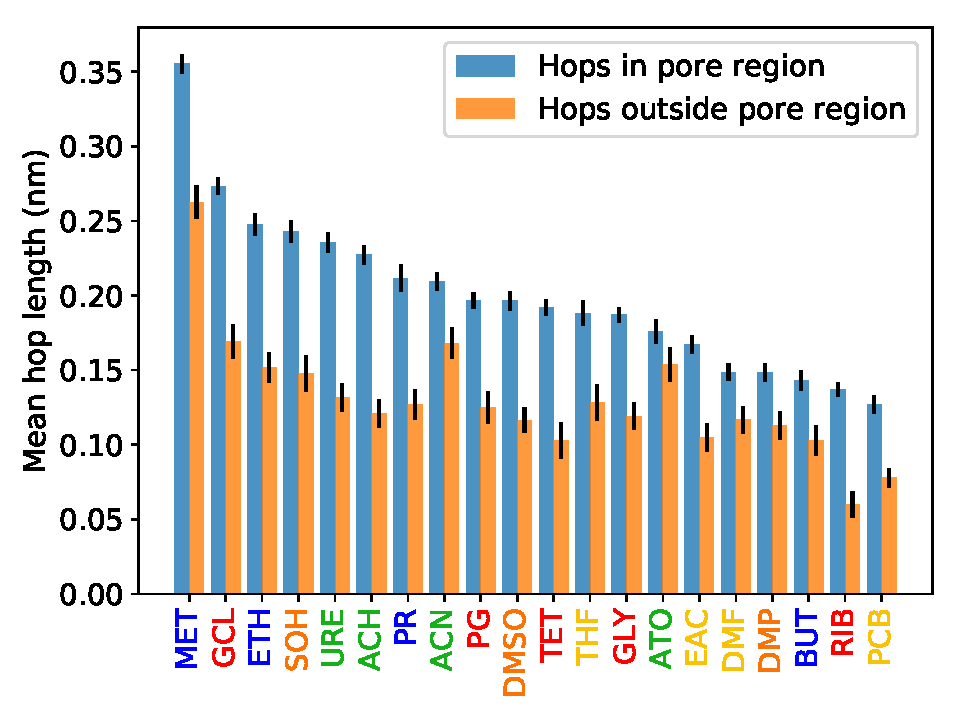
\includegraphics[width=\linewidth]{hop_length.pdf}
  \caption{}\label{fig:hop_lengths}
  \end{subfigure}
  \begin{subfigure}{0.325\textwidth}
  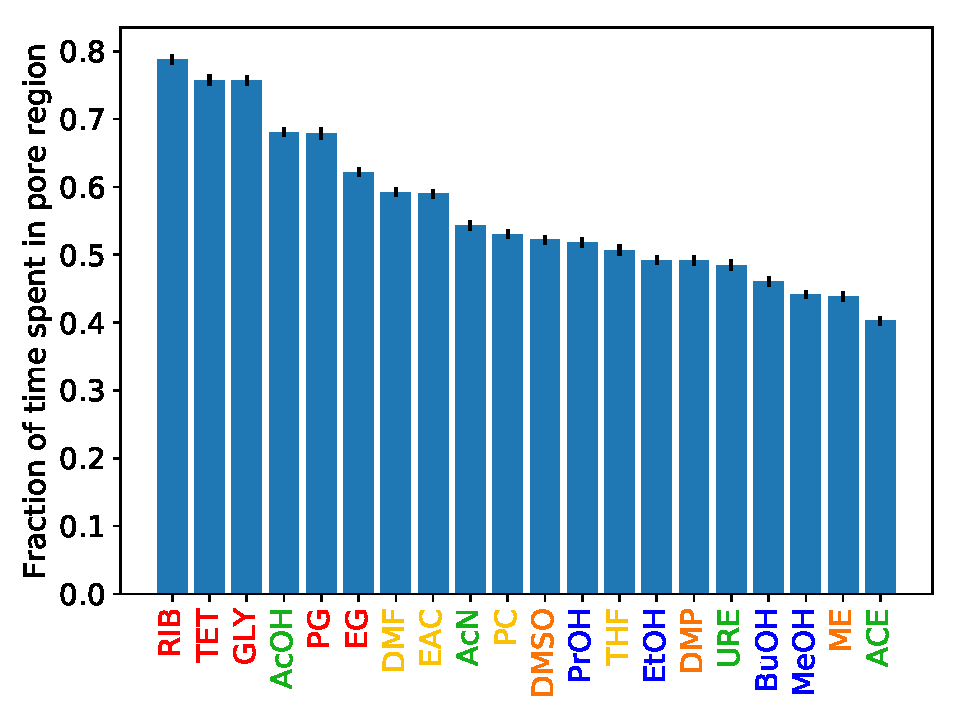
\includegraphics[width=\textwidth]{frac_time_spent.pdf}
  \caption{}\label{fig:frac_time}
  \end{subfigure}
  \begin{subfigure}{0.325\textwidth}
  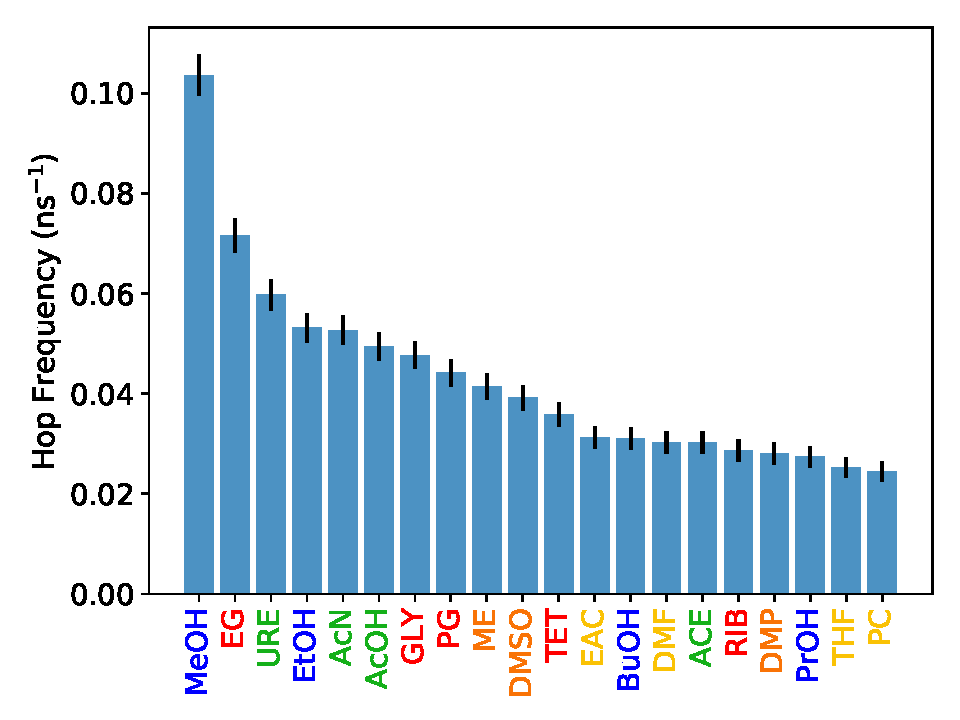
\includegraphics[width=\textwidth]{hopfreq_total.pdf}
  \caption{}\label{fig:hopfreq}
  \end{subfigure}
  \caption{(a) Hops made in the pore region of the 10 wt\% water system
  are, on average, 59 \% larger than those made outside the pore region.
  The trend in hop lengths is similar to the trend in MSDs shown in
  Figure~\ref{fig:all_msds_10wt} implying that solutes which make consistently
  larger hops have higher MSDs. The fraction of time spent by a solute in the
  pore region (b) does not necessarily lead to more frequent hopping (c). For
  example, ribose spends the largest fraction of time in the pore region, yet
  performs the the fifth lowest number of hops.}\label{fig:hops}
  \end{figure}
  
  \noindent The frequency with which solutes donate hydrogen bonds to monomer
  head groups is related to the number of hydrogen bond donating atoms as well
  as their identity.
  \begin{itemize}
    \item The percentage of solutes actively participating in at least one
    hydrogen bond with a head group each frame descends as the number of 
    hydroxyl groups decreases.
    \item Solutes with many hydroxyl groups, such as ribose, tetrose and 
    glycerol, can donate multiple hydrogen bonds to monomer head groups 
    simultaneously. 
    \item When one hydrogen bond is broken, other hydrogen bonds work to
    hold the solute in place, which allows broken hydrogen bonds to reform.
    \item Solutes that containing sulfur and nitrogen atoms in place of 
    oxygen atoms hydrogen bond less frequently since they are less 
    electronegative elements. % citation
    \item The lifetime of hydrogen bonds follows nearly the same trend. Hydrogen
    bonds of solutes that hydrogen bond more frequently last longer. 
  \end{itemize}
  
  \begin{figure}[!htb]
  \centering
  \begin{subfigure}{0.45\textwidth}
  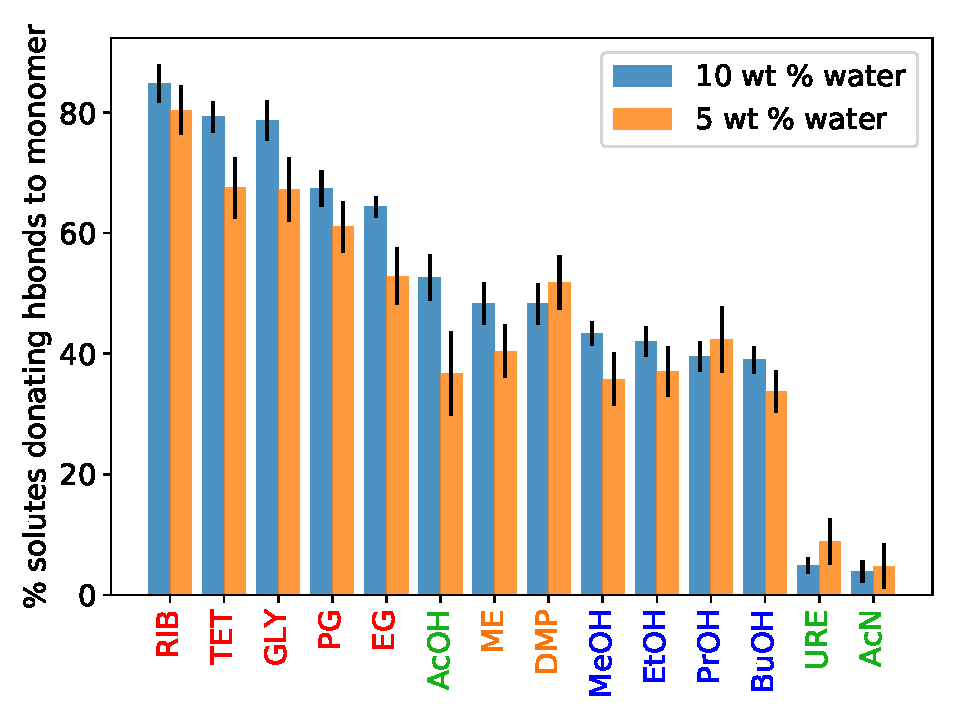
\includegraphics[width=\textwidth]{nhbonds_all.pdf}  % unique_hbonds.py
  \caption{}\label{fig:nhbonds}
  \end{subfigure}
  \begin{subfigure}{0.45\textwidth}
  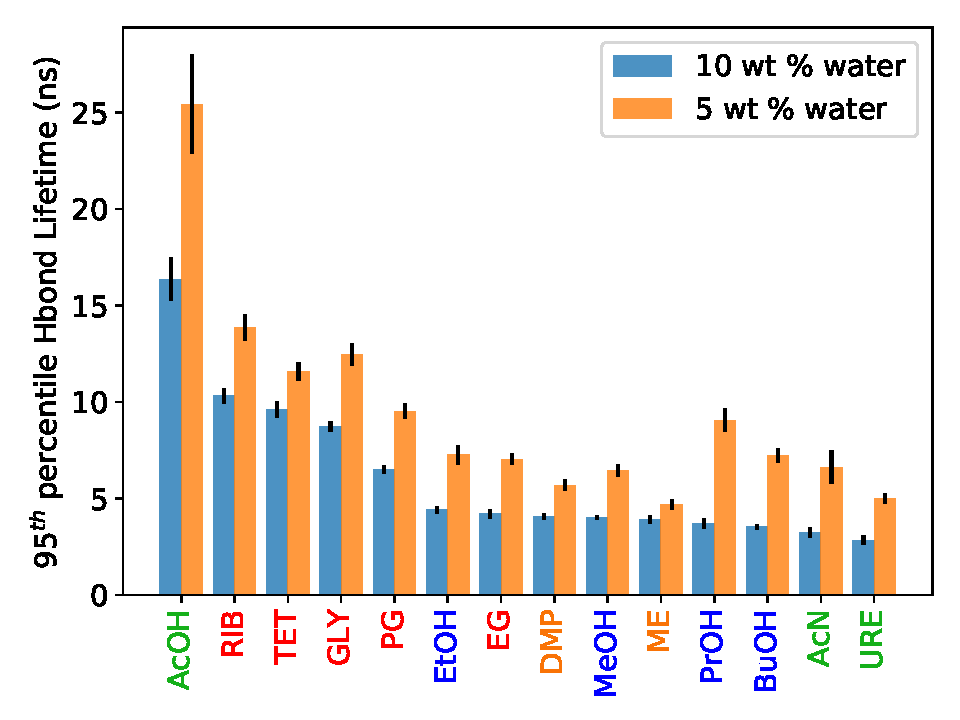
\includegraphics[width=\textwidth]{hbond_lifetime.pdf}  % hbond_dwells.py
  \caption{}\label{fig:hbond_dwells}
  \end{subfigure}
  \caption{(a) Solutes capable of donating hydrogen bonds to monomer head groups
  do so to varying degrees. The reported percentages represent unique solute-monomer
  hydrogen bonds. Individual solutes that hydrogen bond with multiple head groups
  simultaneously are only counted once. (b) The lifetime of individual hydrogen
  bonds appears correlated to the percentage of solutes involved in hydrogen bond
  interactions. Hydrogen bond lifetimes tend to be longer for solutes that
  hydrogen bond frequently. Note that solutes incapable of donating hydrogen
  bonds are omitted from this figure.}\label{fig:hbonds}
  \end{figure}
  
  \noindent Solutes with carbonyl groups tend to associate with sodium ions most frequently.
  \begin{itemize}
    \item Nearly all of the most coordinated solutes contain a carbonyl group 
    (except for DMSO which has an analogous sulfinyl group). 
    \item There is a significant drop in sodium ion association for solutes 
    that do not contain carbonyl groups or multiple hydroxyl groups to compensate 
    (see Figure~\ref{fig:all_solutes_NA_coordination}).
    \item The corresponding dwell times follow a similar trend, however the dwell
    times of highly coordinated solutes with multiple hydroxyl groups are generally
    lower since association between hydroxyl groups and sodium is apparently a 
    weaker interaction (Figure~\ref{fig:all_NA_dwells}).
	\item Solutes with nitrogen atoms adjacent to the carbonyl groups tend to
	associate with sodium ions significantly more. 
  \end{itemize}
  
  \begin{figure}[!htb]
  \centering
  \begin{subfigure}{0.45\textwidth}
  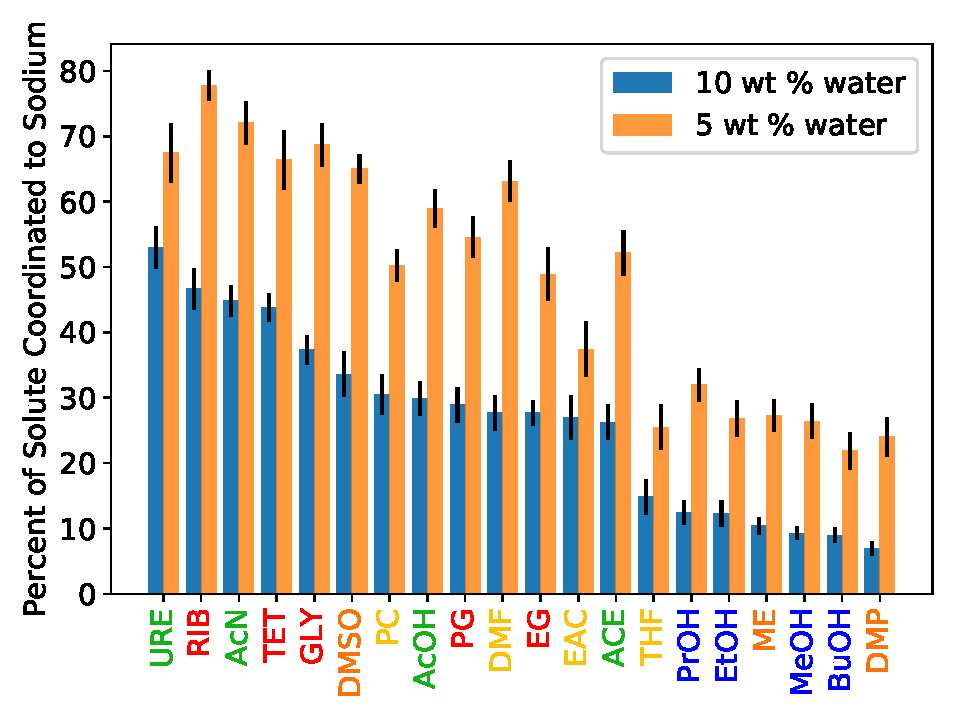
\includegraphics[width=\textwidth]{all_solutes_NA_coordination.pdf}
  \caption{}\label{fig:all_solutes_NA_coordination}
  \end{subfigure}
  \begin{subfigure}{0.45\textwidth}
  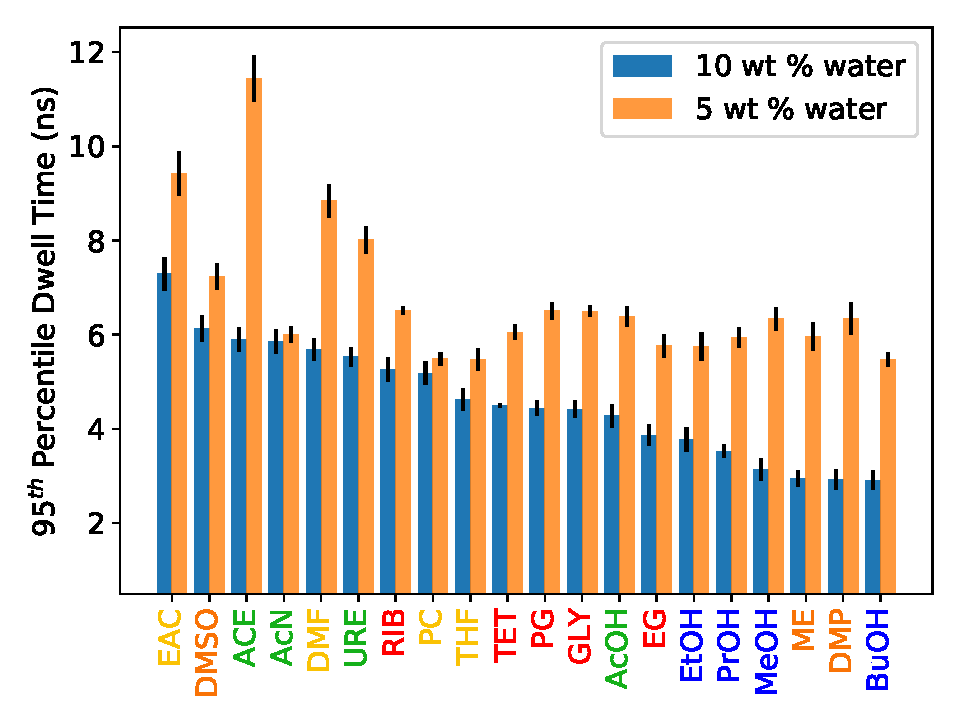
\includegraphics[width=\textwidth]{all_NA_dwells.pdf}
  \caption{}\label{fig:all_NA_dwells}
  \end{subfigure}
  \caption{(a) Solutes, especially those with carbonyl groups, spend a
  significant fraction of time coordinated to sodium ions. (b) The length
  of time a solute-sodium pairs spends associated tends to be higher for
  pairs that associate more frequently.}\label{fig:na_coordination}
  \end{figure}
  
  \noindent \textbf{\large Objective 3:} \textit{\large Create a stochastic model} (\textcolor{blue}{\textbf{In Progress}})
  %MRS: yes, needs to be longer.  you can cut back some of the details in objectives 1 and 2. 
  %BJC: This section will get developed further as I think about it more after the paper is submitted
  \noindent We are in the process of developing the theory required to build a 
  stochastic model. 
  
  \noindent The distribution of dwell times is power law distributed.
  
  \noindent The distribution of hop lengths is approximately Gaussian
  
  \noindent The model will likely have a radial dependence. 
  
  \noindent \textbf{\large Objective 4:} \textit{\large Apply analyses to Q\textsubscript{I} phase} (\textcolor{blue}{\textbf{In Progress}})
  
  Paralleling our work on the H\textsubscript{II} phase, our first task was to
  build a suitable unit cell representation of the Q\textsubscript{I} phase. 
  \begin{itemize}
    \item Unfortunately, the true space group of the Q\textsubscript{I}
    phase that we are studying is unknown. 
    \item Experimental diffraction has narrowed down the possible bicontinuous
    cubic configurations to the Ia3d and Pn3m space groups. 
    \item Therefore, we will build both types of unit cells and search for
    cues that can be used to differentiate them experimentally.
  \end{itemize}  
  
  \noindent We have developed procedures to build both Ia3d and Pn3m unit
  cells.
  \begin{itemize}
    \item To our knowledge, nobody has ever built an atomistic bicontinuous
    cubic phase system without the aid of self-assembly.
    \item Self-assembly can be a long process, especially for fully atomistic
    systems. 
    \item Instead, we used known analytical equations that describe the 
    surface of these systems in order to place monomers into a unit cell.
    \item Monomers are placed perpendicular to the surface in random locations
    that don't overlap. One can control the pore size by translating monomers 
    perpendicular to the surface at the point where they are attached.
    %BJC: not sure how much more detail to include. Can go into a lot. Have to expand box and slowly compress. Add glycerol iteratively until there are no gaps.
  \end{itemize}
  
%  \noindent \textbf{\large Objective 5} \textit{\large Create a well-documented python package} (\textcolor{blue}{\textbf{In Progress}})
%  
%  Python scripts used to simulate X-ray diffraction patterns are available in the following
%  GitHub repository: \url{https://github.com/joeyelk/MD-Structure-Factor}. Documentation
%  is forthcoming. 
%  
%  Python scripts used to conduct all other post-simulation trajectory analysis are 
%  also available on GitHub: \url{https://github.com/shirtsgroup/LLC_Membranes}. 
%  Documentation is a work in progress. It is available for viewing in its 
%  current state at \url{https://llc-membranes.readthedocs.io/en/latest/}.

  \section{Timeline for Completion of Objectives}\label{section:timeline}

  A schematic of the estimated timeline that will be followed for the completion of
  tasks pertinent to finishing all objectives is given in Table~\ref{table:timeline}.
  \begin{itemize}
    \item Simulations required to study the structure of the bicontinuous cubic
    phase will be run in parallel while working out the details of our stochastic
    model of transport in the H\textsubscript{II} phase.
    \item Simulations and analysis required for Q\textsubscript{I} phase solute 
    transport studies analogous to those of Objective 2 will be carried out 
    throughout Fall 2019.
    \item Finalization of code documentation and application of a stochastic
    model to the Q\textsubscript{I} phase will be finished by May 2020
  \end{itemize}

  \begin{center}  
  \begin{table}[!htb]
	\renewcommand\arraystretch{1.4}\arrayrulecolor{LightSteelBlue3}
	\captionsetup{singlelinecheck=false, font=blue, labelfont=sc, labelsep=quad}
	\caption{Estimated Timeline for Completion of Objectives}\vskip -1.5ex
	\begin{tabular}{@{\,}r <{\hskip 2pt} !{\foo} >{\raggedright\arraybackslash}p{8cm}}
	\toprule
	\addlinespace[1.5ex]
	August 2019 & Complete Stochastic Model for H\textsubscript{II} phase \\
	September 2019 & Finalize Q\textsubscript{I} phase structure \\
    January 2020 & Finish transport study of Q\textsubscript{I} phase \\
    April 2020 & Complete code documentation \\
    April 2020 & Finish application of stochastic model to Q\textsubscript{I} phase \\
    May 2020 & PhD Defense \\
	\end{tabular}
	\label{table:timeline}
  \end{table}
  \end{center}
  
  \section{Resource Requirements}\label{section:resources}
  %BJC: Not sure what to include here. Hour estimate? Or omit this section.   
  
  The remainder of our work will require the use of high performance computing (HPC)
  resources. 
  \begin{itemize}
    \item We will continue using Bridges, an XSEDE resource as well as Summit, a
    supercomputer located at CU Boulder.
  \end{itemize}
  
  % BJC: add funding?

  \newpage
  \bibliographystyle{ieeetr}
  \bibliography{comps}

\end{document}
